%==============================================================================
% Tento soubor použijte jako základ
% This file should be used as a base for the thesis
% Autoři / Authors: 2008 Michal Bidlo, 2022 Jaroslav Dytrych
% Kontakt pro dotazy a připomínky: sablona@fit.vutbr.cz
% Contact for questions and comments: sablona@fit.vutbr.cz
%==============================================================================
% kódování: UTF-8 (zmena prikazem iconv, recode nebo cstocs)
% encoding: UTF-8 (you can change it by command iconv, recode or cstocs)
%------------------------------------------------------------------------------
% zpracování / processing: make, make pdf, make clean
%==============================================================================
% Soubory, které je nutné upravit nebo smazat: / Files which have to be edited or deleted:
%   projekt-20-literatura-bibliography.bib - literatura / bibliography
%   projekt-01-kapitoly-chapters.tex - obsah práce / the thesis content
%   projekt-01-kapitoly-chapters-en.tex - obsah práce v angličtině / the thesis content in English
%   projekt-30-prilohy-appendices.tex - přílohy / appendices
%   projekt-30-prilohy-appendices-en.tex - přílohy v angličtině / appendices in English
%==============================================================================
\documentclass[slovak,zadani]{fitthesis} % bez zadání - pro začátek práce, aby nebyl problém s překladem
%\documentclass[english]{fitthesis} % without assignment - for the work start to avoid compilation problem
%\documentclass[zadani]{fitthesis} % odevzdani do IS VUT a/nebo tisk s barevnými odkazy - odkazy jsou barevné
%\documentclass[english,zadani]{fitthesis} % for submission to the IS VUT and/or print with color links - links are color
%\documentclass[zadani,print]{fitthesis} % pro černobílý tisk - odkazy jsou černé
%\documentclass[english,zadani,print]{fitthesis} % for the black and white print - links are black
%\documentclass[zadani,cprint]{fitthesis} % pro barevný tisk - odkazy jsou černé, znak VUT barevný
%\documentclass[english,zadani,cprint]{fitthesis} % for the print - links are black, logo is color
% * Je-li práce psaná v anglickém jazyce, je zapotřebí u třídy použít 
%   parametr english následovně:
%   If thesis is written in English, it is necessary to use 
%   parameter english as follows:
%      \documentclass[english]{fitthesis}
% * Je-li práce psaná ve slovenském jazyce, je zapotřebí u třídy použít 
%   parametr slovak následovně:
%   If the work is written in the Slovak language, it is necessary 
%   to use parameter slovak as follows:
%      \documentclass[slovak]{fitthesis}
% * Je-li práce psaná v anglickém jazyce se slovenským abstraktem apod., 
%   je zapotřebí u třídy použít parametry english a enslovak následovně:
%   If the work is written in English with the Slovak abstract, etc., 
%   it is necessary to use parameters english and enslovak as follows:
%      \documentclass[english,enslovak]{fitthesis}

% Základní balíčky jsou dole v souboru šablony fitthesis.cls
% Basic packages are at the bottom of template file fitthesis.cls
% zde můžeme vložit vlastní balíčky / you can place own packages here


% Pro seznam zkratek lze využít balíček Glossaries - nutno odkomentovat i níže a při kompilaci z konzoly i v Makefile (plnou verzi pro Perl, nebo lite)
% The Glossaries package can be used for the list of abbreviations - it is necessary to uncomment also below. When compiling from the console also in the Makefile (full version for Perl or lite)
%\usepackage{glossaries}
%\usepackage{glossary-superragged}
%\makeglossaries 

% Nastavení cesty k obrázkům
% Setting of a path to the pictures
%\graphicspath{{obrazky-figures/}{./obrazky-figures/}}
%\graphicspath{{obrazky-figures/}{../obrazky-figures/}}

%---rm---------------
\renewcommand{\rmdefault}{lmr}%zavede Latin Modern Roman jako rm / set Latin Modern Roman as rm
%---sf---------------
\renewcommand{\sfdefault}{qhv}%zavede TeX Gyre Heros jako sf
%---tt------------
\renewcommand{\ttdefault}{lmtt}% zavede Latin Modern tt jako tt

% vypne funkci šablony, která automaticky nahrazuje uvozovky,
% aby nebyly prováděny nevhodné náhrady v popisech API apod.
% disables function of the template which replaces quotation marks
% to avoid unnecessary replacements in the API descriptions etc.
\csdoublequotesoff

\usepackage{url}

% =======================================================================
% balíček "hyperref" vytváří klikací odkazy v pdf, pokud tedy použijeme pdflatex
% problém je, že balíček hyperref musí být uveden jako poslední, takže nemůže
% být v šabloně
% "hyperref" package create clickable links in pdf if you are using pdflatex.
% Problem is that this package have to be introduced as the last one so it 
% can not be placed in the template file.
\ifWis
\ifx\pdfoutput\undefined % nejedeme pod pdflatexem / we are not using pdflatex
\else
  \usepackage{color}
  \usepackage[unicode,colorlinks,hyperindex,plainpages=false,pdftex]{hyperref}
  \definecolor{hrcolor-ref}{RGB}{223,52,30}
  \definecolor{hrcolor-cite}{HTML}{2F8F00}
  \definecolor{hrcolor-urls}{HTML}{092EAB}
  \hypersetup{
	linkcolor=hrcolor-ref,
	citecolor=hrcolor-cite,
	filecolor=magenta,
	urlcolor=hrcolor-urls
  }
  \def\pdfBorderAttrs{/Border [0 0 0] }  % bez okrajů kolem odkazů / without margins around links
  \pdfcompresslevel=9
\fi
\else % pro tisk budou odkazy, na které se dá klikat, černé / for the print clickable links will be black
\ifx\pdfoutput\undefined % nejedeme pod pdflatexem / we are not using pdflatex
\else
  \usepackage{color}
  \usepackage[unicode,colorlinks,hyperindex,plainpages=false,pdftex,urlcolor=black,linkcolor=black,citecolor=black]{hyperref}
  \definecolor{links}{rgb}{0,0,0}
  \definecolor{anchors}{rgb}{0,0,0}
  \def\AnchorColor{anchors}
  \def\LinkColor{links}
  \def\pdfBorderAttrs{/Border [0 0 0] } % bez okrajů kolem odkazů / without margins around links
  \pdfcompresslevel=9
\fi
\fi
% Řešení problému, kdy klikací odkazy na obrázky vedou za obrázek
% This solves the problems with links which leads after the picture
\usepackage[all]{hypcap}


% Informace o práci/projektu / Information about the thesis
%---------------------------------------------------------------------------
\projectinfo{
  %Prace / Thesis
  project={BP},            %typ práce BP/SP/DP/DR  / thesis type (SP = term project)
  year={2024},             % rok odevzdání / year of submission
  date=\today,             % datum odevzdání / submission date
  %Nazev prace / thesis title
  title.cs={VIRTUÁLNÍ LABORATOŘ PRO PYNQ},  % název práce v češtině či slovenštině (dle zadání) / thesis title in czech language (according to assignment)
  title.en={Remote laboratory for PYNQ}, % název práce v angličtině / thesis title in english
  %title.length={14.5cm}, % nastavení délky bloku s titulkem pro úpravu zalomení řádku (lze definovat zde nebo níže) / setting the length of a block with a thesis title for adjusting a line break (can be defined here or below)
  %sectitle.length={14.5cm}, % nastavení délky bloku s druhým titulkem pro úpravu zalomení řádku (lze definovat zde nebo níže) / setting the length of a block with a second thesis title for adjusting a line break (can be defined here or below)
  %dectitle.length={14.5cm}, % nastavení délky bloku s titulkem nad prohlášením pro úpravu zalomení řádku (lze definovat zde nebo níže) / setting the length of a block with a thesis title above declaration for adjusting a line break (can be defined here or below)
  %Autor / Author
  author.name={Boris},   % jméno autora / author name
  author.surname={Veselý},   % příjmení autora / author surname 
  %author.title.p={Bc.}, % titul před jménem (nepovinné) / title before the name (optional)
  %author.title.a={Ph.D.}, % titul za jménem (nepovinné) / title after the name (optional)
  %Ustav / Department
  department={UPSY}, % doplňte příslušnou zkratku dle ústavu na zadání: UPSY/UIFS/UITS/UPGM / fill in appropriate abbreviation of the department according to assignment: UPSY/UIFS/UITS/UPGM
  % Školitel / supervisor
  supervisor.name={Vojtěch},   % jméno školitele / supervisor name 
  supervisor.surname={Mrázek},   % příjmení školitele / supervisor surname
  supervisor.title.p={Ing.},   %titul před jménem (nepovinné) / title before the name (optional)
  supervisor.title.a={Ph.D.},    %titul za jménem (nepovinné) / title after the name (optional)
  % Klíčová slova / keywords
  keywords.cs={virtuálne laboratórium, FPGA, Zynq, PYNQ, rezervačný systém, PHP, Nette, Go, JavaScript, démon, tunel, maškaráda, presmerovanie komunikácie, REST API, webová aplikácia}, % klíčová slova v českém či slovenském jazyce / keywords in czech or slovak language
  keywords.en={remote lab, FPGA, Zynq, PYNQ, reservation system, PHP, Nette, Go, JavaScript, daemon, tunnel, masquerade, communication redirection, REST API, web application}, % klíčová slova v anglickém jazyce / keywords in english
  %keywords.en={Here, individual keywords separated by commas will be written in English.},
  % Abstrakt / Abstract
  abstract.cs={Táto práca slúži na~poskytovanie zariadení PYNQ viacerým používateľom na výučbu predmetu IVH. Aplikácia virtuálneho laboratória poskytuje prístup k~zariadeniam PYNQ pomocou tunelových spojení. V~aplikácii je možné spravovať súbory uložené na serveri a~registrovať si časové úseky, počas ktorých bude používateľovi umožnený prístup ku zariadeniam PYNQ pomocou tunelových spojení. Aplikácia umožňuje aj rolu administrátora, ktorý môže spravovať používateľov, ich rezervácie a~jednotlivé zariadenia PYNQ. Aplikácia je napísaná pomocou jazykov PHP, rámca Nette a~Go. Prínosom práce je zjednodušenie prístupu ku zariadeniam PYNQ v~rámci výučby predmetu IVH.}, % abstrakt v českém či slovenském jazyce / abstract in czech or slovak language
  abstract.en={This thesis is used to~provide PYNQ devices to multiple users for teaching the IVH subject. The remote laboratory application provides access to the PYNQ devices using tunnel connections. The application can manage the files stored on the server and register the time slots during which the user will be allowed to access the PYNQ devices using tunnel connections. The application also allows an administrator role that can manage users, their reservations and individual PYNQ devices. The application is written using PHP, the Nette framework and Go. The contribution of the work is to simplify access to PYNQ devices in~the context of teaching the IVH subject.}, % abstrakt v anglickém jazyce / abstract in english
  %abstract.en={An abstract of the work in English will be written in this paragraph.},
  % Prohlášení (u anglicky psané práce anglicky, u slovensky psané práce slovensky; u projektové praxe lze zakomentovat) / Declaration (for thesis in english should be in english; for project practice can be commented out)
  declaration={Prehlasujem, že som túto bakalársku prácu vypracoval samostatne pod vedením pána Ing.~Vojtěcha Mrázeka, Ph.D. 
  Uviedol som všetky literárne pramene, publikácie a ďalšie zdroje, z ktorých som čerpal.},
  %declaration={I hereby declare that this Bachelor's thesis was prepared as an original work by the author under the supervision of Mr. X
% The supplementary information was provided by Mr. Y
% I have listed all the literary sources, publications and other sources, which were used during the preparation of this thesis.},
  % Poděkování (nepovinné, nejlépe v jazyce práce; nechcete-li, zakomentujte pro skrytí nadpisu) / Acknowledgement (optional, ideally in the language of the thesis; comment out for hiding including heading)
  acknowledgment={Chcel by som sa poďakovať môjmu vedúcemu práce Ing.~Vojtěchovi Mrázekovi, Ph.D., ktorý mi poskytol odbornú pomoc pri písaní tejto práce. Ďalej by som sa chcel poďakovať mojej rodine a blízkemu kruhu priateľov, ktorí mi boli oporou počas celého štúdia.},
  %acknowledgment={Here it is possible to express thanks to the supervisor and to the people which provided professional help
%(external submitter, consultant, etc.).},
  % Rozšířený abstrakt (cca 3 normostrany) - lze definovat zde nebo níže / Extended abstract (approximately 3 standard pages) - can be defined here or below
  %extendedabstract={Do tohoto odstavce bude zapsán rozšířený výtah (abstrakt) práce v českém (slovenském) jazyce.},
  %extabstract.odd={true}, % Začít rozšířený abstrakt na liché stránce? / Should extended abstract start on the odd page?
  %faculty={FIT}, % FIT/FEKT/FSI/FA/FCH/FP/FAST/FAVU/USI/DEF
  faculty.cs={Fakulta informačních technologií}, % Fakulta v češtině - pro využití této položky výše zvolte fakultu DEF / Faculty in Czech - for use of this entry select DEF above
  faculty.en={Faculty of Information Technology}, % Fakulta v angličtině - pro využití této položky výše zvolte fakultu DEF / Faculty in English - for use of this entry select DEF above
  department.cs={Ústav matematiky}, % Ústav v češtině - pro využití této položky výše zvolte ústav DEF nebo jej zakomentujte / Department in Czech - for use of this entry select DEF above or comment it out
  department.en={Institute of Mathematics} % Ústav v angličtině - pro využití této položky výše zvolte ústav DEF nebo jej zakomentujte / Department in English - for use of this entry select DEF above or comment it out
}

% Rozšířený abstrakt (cca 3 normostrany) - lze definovat zde nebo výše / Extended abstract (approximately 3 standard pages) - can be defined here or above
%\extendedabstract{Do tohoto odstavce bude zapsán výtah (abstrakt) práce v českém (slovenském) jazyce.}
% Začít rozšířený abstrakt na liché stránce? / Should extended abstract start on the odd page?
%\extabstractodd{true}

% nastavení délky bloku s titulkem pro úpravu zalomení řádku - lze definovat zde nebo výše / setting the length of a block with a thesis title for adjusting a line break - can be defined here or above
%\titlelength{14.5cm}
% nastavení délky bloku s druhým titulkem pro úpravu zalomení řádku - lze definovat zde nebo výše / setting the length of a block with a second thesis title for adjusting a line break - can be defined here or above
%\sectitlelength{14.5cm}
% nastavení délky bloku s titulkem nad prohlášením pro úpravu zalomení řádku - lze definovat zde nebo výše / setting the length of a block with a thesis title above declaration for adjusting a line break - can be defined here or above
%\dectitlelength{14.5cm}

% řeší první/poslední řádek odstavce na předchozí/následující stránce
% solves first/last row of the paragraph on the previous/next page
\clubpenalty=10000
\widowpenalty=10000

% checklist
\newlist{checklist}{itemize}{1}
\setlist[checklist]{label=$\square$}

% Kompilace po částech (rychlejší, ale v náhledu nemusí být vše aktuální)
% Compilation piecewise (faster, but not all parts in preview will be up-to-date)
% Další informace viz / For more information see https://www.overleaf.com/learn/latex/Multi-file_LaTeX_projects
% \usepackage{subfiles}

% Nechcete-li, aby se u oboustranného tisku roztahovaly mezery pro zaplnění stránky, odkomentujte následující řádek / If you do not want enlarged spacing for filling of the pages in case of duplex printing, uncomment the following line
% \raggedbottom

\begin{document}
  % Vysazeni titulnich stran / Typesetting of the title pages
  % ----------------------------------------------
  \maketitle
  % Obsah
  % ----------------------------------------------
  \setlength{\parskip}{0pt}

  \setcounter{tocdepth}{1}

  {\hypersetup{hidelinks}\tableofcontents}
  
  % Seznam obrazku a tabulek (pokud prace obsahuje velke mnozstvi obrazku, tak se to hodi)
  % List of figures and list of tables (if the thesis contains a lot of pictures, it is good)
  % \ifczech
  %   \renewcommand\listfigurename{Seznam obrázků}
  % \fi
  % \ifslovak
  %   \renewcommand\listfigurename{Zoznam obrázkov}
  % \fi
  % {\hypersetup{hidelinks}\listoffigures}
  
  % \ifczech
  %   \renewcommand\listtablename{Seznam tabulek}
  % \fi
  % \ifslovak
  %   \renewcommand\listtablename{Zoznam tabuliek}
  % \fi
  % {\hypersetup{hidelinks}\listoftables}

  % Seznam zkratek / List of abbreviations
  %\ifczech
  %  \renewcommand*\glossaryname{Seznam zkratek}%
  %  \renewcommand*\entryname{Zkratka}
  %  \renewcommand*\descriptionname{Význam}
  %\fi
  %\ifslovak
  %  \renewcommand*\glossaryname{Zoznam skratiek}%
  %  \renewcommand*\entryname{Skratka}
  %  \renewcommand*\descriptionname{Význam}
  %\fi
  %\ifenglish
  %  \renewcommand*\glossaryname{List of abbreviations}%
  %  \renewcommand*\entryname{Abbreviation}
  %  \renewcommand*\descriptionname{Meaning}
  %\fi
  % Definice zkratek - z textu se odkazují např. \Gls{TF–IDF}
  % Definition of abbreviations - referred from the text e.g. \Gls{TF–IDF}
  %\newglossaryentry{TF–IDF}
  %{
  %  name={TF–IDF},
  %  description={Term Frequency-Inverse Document Frequency}
  %}
  % 
  %\setglossarystyle{superragged}
  %\printglossaries


  \ifODSAZ
    \setlength{\parskip}{0.5\bigskipamount}
  \else
    \setlength{\parskip}{0pt}
  \fi

  % vynechani stranky v oboustrannem rezimu
  % Skip the page in the two-sided mode
  \iftwoside
    \cleardoublepage
  \fi

  % Text prace / Thesis text
  % ----------------------------------------------
  \ifenglish
    \input{projekt-01-kapitoly-chapters-en}
  \else
    \chapter{Úvod}

Na výučbu na fakulte sa používajú fyzické zariadenia Zynq s~nadstavbou PYNQ, ktoré si každý študent musí vypožičať a~každé zariadenie musí byť nastavené lektorom vyučovaného predmetu. Čo vytvára prácu naviac pre lektora aj pre študenta. Táto práca naviac by sa dala minimalizovať vytvorením systému, do ktorého by mali prístup študenti a~lektori, ktorý by poskytoval prístup cez webový prehliadač k~týmto zariadeniam, čím by bolo študentom umožnené pracovať so zariadeniami v~rezervovaných časových úsekoch.   

Táto práca slúži na poskytovanie zariadení PYNQ viacerým používateľom na výučbu predmetu IVH. Na týchto zariadenia si používatelia testujú svoje projekty. Preto bolo cieľom práce nájsť spôsob a~vytvoriť aplikáciu, ktorá umožní používateľom férový a~bezpečný prístup ku zdielaným zariadeniam, čím sa umožní používateľom takmer neobmedzený prístup k~zariadeniam a~to bez nutnosti ich vypožičania.

Pre aplikáciu je dôležité, aby každý používateľ mal férový prístup do systému, kde si môže vytvoriť rezerváciu na daný časový úsek, počas ktorého môže neprerušovane a~bezpečne pracovať so zariadením PYNQ. Je dôležité, aby aplikácia bola bezpečná a~neumožňovala používateľovi prístup k~dátam iného používateľa, alebo prístup viacerým používateľom naraz k~jednému zariadeniu. Aplikácia bude poskytovať rozhranie ako pre obyčajných používateľov, tak aj pre lektora, ktorý bude môcť v~aplikácii vykonávať administratívne úlohy.

Nasledujúca kapitola \ref{prostriedky} sa venuje problematike zdieľania prostriedkov viacerým používateľom, kde sú popísané možnosti, ako sa dajú dané prostriedky zdieľať. Kapitola \ref{Zynq}. popisuje dosky ZYNQ a~ich nadstavby PYNQ, kde je popísaná ich architektúra, ako fungujú a~prečo môžu byť dobré pre výučbu hardvéru popisného jazyka. V kapitole \ref{Navrh} je riešený návrh samotného systému aplikácie virtuálneho laboratória pre študentov. Konkrétna implementácia tejto aplikácie je následne riešená v~kapitole \ref{Implementacia}. Posledná kapitola \ref{testovanie} sa venuje otestovaniu systému na vzorke používateľov a~následnému vyhodnoteniu vlastností implementovaného systému.

\chapter{Zdieľanie prostriedkov viacerým užívateľom}
\label{prostriedky}

Ak chce používateľ zdielať prostriedky viacerým používateľom, môže ich zdieľať pomocou niekoľkých možných implementácií. Napríklad pomocou zhlukov komoditných počítačov a~plánovacích frontov, ktoré vystupujú ako jeden systém, do ktorého je nahraná úloha, ktorá je zaradená do frontu, systém túto úlohu vykoná a~používateľ dostane výsledok vykonania tejto úlohy. Ďalej môže používateľ tieto prostriedky zdieľať pomocou rezervácií jednotlivých časových úsekov v~rámci virtuálneho laboratória, v~ktorom si používateľ rezervuje a~počas tohto časového úseku je mu pridelené zariadenie z~daného virtuálneho laboratória, na ktorom môže vykonávať prácu. Používatelia sa takto môžu jednoducho striedať a~nie je potrebné implementovať napríklad ďalej popísaný algoritmus na určenie poradia úloh vo frontoch, ale je potrebné zabezpečiť iné opatrenia systému.

\section{Prenosný dávkový systém}

Zhluky komoditných počítačov sa objavili ako hlavne paralelné a~distribuované platformy pre vysoko výkonné a~vysoko dostupné výpočtové systémy. Sú prezentované spoločne ako jeden zjednotený zdroj pre koncových používateľov pomocou middlewarových technológií, ako je správa zdrojov a~plánovací systém. Používatelia odosielajú úlohy v~dávkach do frontu systému správy zdrojov a~centralizovaný plánovač rozhodne, ako uprednostniť a~prideliť prostriedky na vykonanie úloh. Plánovače by mali byť schopné poskytnúť signál spätnej väzby, ktorý používateľom bráni v~odosielaní neobmedzeného množstva práce.~\cite{SherwaniJahanzeb2004Lace}

Prenosný dávkový systém (Portable batch system - PBS) je flexibilný, POSIX kompatibilný systém dávkového zaraďovania a~riadenia pracovného zaťaženia. Funguje na sieťových, multiplatformových prostrediach UNIX, vrátane heterogénnych zhlukov pracovných staníc, superpočítačov a~masívne paralelných systémov. Tento projekt bol iniciovaný s~cieľom vytvoriť flexibilný, rozšíriteľný systém dávkového spracovania, ktorý spĺňa jedinečné požiadavky heterogénnych počítačových sietí. Účelom PBS je poskytnúť dodatočné kontroly nad inicializáciou, alebo plánovaním vykonávania dávkových úloh a~umožniť smerovanie týchto úloh medzi rôznymi hostiteľmi. Má tiež priateľské grafické rozhranie.~\cite{SherwaniJahanzeb2004Lace}

\subsection{Fronty a~plánovanie}

Predvolený plánovač v~PBS je FIFO, ktorého správaním je maximalizovať využitie CPU. To znamená, že prechádza zoznamom úloh vo fronte a~spúšťa akúkoľvek úlohu, ktorá sa zmestí do dostupných zdrojov. Toto však účinne zabraňuje tomu, aby sa veľké úlohy vôbec spustili. Aby sa umožnilo spustenie veľkých úloh, tento plánovač implementuje mechanizmus „hladujúcich úloh“. Táto metóda môže fungovať v~niektorých situáciách, ale existujú určité okolnosti, kedy tento postup neprináša požadované výsledky. V~tomto čase prichádzajú do hry alternatívne plánovače, ktoré možno použiť s~PBS.~\cite{SherwaniJahanzeb2004Lace}

Výber politiky plánovania práce môže ovplyvniť čas, kedy sa úlohy používateľa začnú vykonávať, a~ďalej ovplyvniť, či používatelia vedia použiť výpočtové zdroje spravodlivo a~rozumne. V~masívne paralelných systémoch spracovania boli algoritmy plánovania úloh kľúčovým faktorom ovplyvňujúcim využitie systémového procesoru.~\cite{HanLuRSAf}

V~súčasnosti sú bežné stratégie plánovania FCFS (First Come First Served), SPT (Shortest Processing Time), First Fit, Best Fit, Greedy a~tak ďalej. V~rámci tradičných zoskupení je tiež veľká základňa práce na plánovaní pracovných miest. Niektoré z~vyspelejších systémov riadenia úloh sú platforma LSF (Load Sharing Facility), PBS Pro, Torque a~Slurm. Neskôr sa objavili vylepšené algoritmy založené na backfillingu a~jemu podobné. Hoci algoritmus backfillingu môže do určitej miery zlepšiť využitie CPU, môže nastať moment, keď nebudú existovať žiadne úlohy, ktoré by zaplnili voľný priestor CPU, keď parametre úlohy vo fronte nemôžu spĺňať podmienky algoritmu Backfilling.~\cite{HanLuRSAf}

\subsection{Problémy a~riešenia}

Každá úloha vstupuje do systému v~určitom čase príchodu tým, že je zaradená do špecifického frontu (v~závislosti od volieb používateľa a~od charakteristík úlohy). Analýzou existujúcich stôp vykonávania pochádzajúcich z~PBS sme určili odhadovaný čas čakania pre každý front, ktorý sa vzťahuje na každú úlohu, ktorú obsahuje. Pri odosielaní úlohy musí používateľ špecifikovať niekoľko informácií, vrátane maximálneho povoleného času vykonania, maximálneho počtu uzlov, ktoré sa majú použiť, a~požadovaných zdrojov (jadrá, pamäť, GPU, MIC). Podľa konvencie systém PBS považuje každú úlohu, ako keby bola rozdelená na súbor presne identických „jednotiek úloh“, ktoré majú byť mapované na jednom uzle. Problém dispečingu vyžaduje priradiť čas začiatku každej čakacej úlohe a~uzol každej z~jej jednotiek. Mali by sa rešpektovať všetky limity kapacity zdrojov a~výkonu, pričom sa zohľadní prítomnosť úloh, ktoré sa už vykonávajú. Jednotlivé aktivity nemajú žiadny konečný termín ani čas vydania (t. j. nemusia skončiť v~určitom dátume alebo začať po určitom dátume), ani celkový rozsah nie je obmedzený žiadnou hornou hranicou. 

Spolu s~vyššie uvedenými zdrojmi v~tomto probléme uvádzame ďalší obmedzený zdroj, výkon. To umožňuje modelovať a~presadzovať obmedzenie výkonu. Úroveň obmedzenia výkonu, t.j. maximálne množstvo energie spotrebovanej systémom v~akomkoľvek danom čase, je špecifikované používateľom a~predstavuje kapacitu falošného zdroja energie; súčet celého výkonu spotrebovaného bežiacou úlohou plus súčet hodnôt výkonu súvisiacich s~nečinnými zdrojmi nesmie nikdy prekročiť daný limit počas vykonávania celého plánu. Ďalšou dôležitou vecou, ktorú si treba všimnúť, je, že „zdroj“ energie nemá lineárne správanie, pokiaľ ide o~výpočtovú záťaž: prvá aktivácia jadra v~uzle spôsobuje väčšiu spotrebu energie pre zostávajúce jadrá v~tomto uzle. Cieľom je skrátiť čakacie doby ako meradlo kvality služieb zaručenej používateľom superpočítačov.~\cite{BorghesiAndrea2015PCiH}

\section{Virtuálne laboratóriá a~časové úseky}

Laboratóriá sú nevyhnutné pre výučbu technologických predmetov, kde sú potrebné praktické experimenty na získanie očakávaných kompetencií a~odborných zručností. Preto virtuálne laboratórium, ktoré poskytne študentovi také isté možnosti ako normálne laboratórium, má veľa výhod. Študenti môžu pracovať doma so svojimi osobnými počítačmi s~jednotlivými operačnými systémami, editormi a~podobne. Majú prístup k~hardvéru laboratória 24 hodín denne. Laboratórium je možné realizovať veľmi kompaktne, čím sa ušetrí veľa miesta a~znížia sa aj náklady na personál. Výhody e-learningových systémov nie sú niečím novým a~v~oblasti strojárstva ho doteraz využíva množstvo iných univerzít.~\cite{reichenbach2011new, monzo2021remote}
Mnohé z~takýchto e-learningových kurzov sú však založené len na teoretickej alebo simulačnej báze. Aby bol zrealizovaný rozumný e-learningový kurz v~oblasti strojárstva a~boli využité vyššie uvedené dôvody, je potrebné vybudovať online laboratórium s programovateľnými hradlovými poľami (field programmable gate arrays - FPGA) pre vzdialený prístup. Jednotlivé FPGA dosky by boli pripojené k~serveru na univerzite a~budú programované serverom. Dosky FPGA budú napríklad monitorované pomocou kamier, aby používatelia videli stav dosiek, napr. blikajúce LED diódy alebo informácie na integrovanom displeji.~\cite{reichenbach2011new}

Na správu online laboratória je potrebný server s~nástrojom na správu zdrojov. Hlavnou výzvou je rozhodnúť o~prístupe mnohých používateľov k~obmedzenému počtu dosiek. Každý študent by mal dostať možnosť používať dosku a~po použití musí byť prístup k~doske uvoľnený pre ďalšieho študenta. Je veľmi dôležité, že neexistuje možnosť blokovania dosky na dlhší čas. Po pevnom časovom úseku by mal mať používateľ napríklad na krátky čas zakázaný prístup k~rezervačnému systému. Rezervačný systém musí byť zabezpečený proti nesprávnemu prístupu a~v~najlepšom prípade využívať bezpečnostné mechanizmy základného operačného systému.~\cite{reichenbach2011new}

\subsection{Rezervácia časových úsekov}

Každá implementácia virtuálneho laboratória má svoj špeciálny rezervačný systém, ktorý umožňuje používateľom rezervovať si časový úsek na prácu na zariadení. Používateľovi je buď umožnený prístup v~časovom úseku ktorý mu vyhradí inštruktor kurzu počas hodín výučby, čo nie je veľmi efektívne. Alebo si teda používateľ pomocou rezervačného systému vytvorí rezerváciu sám na inštruktorom predom definovaný čas, počas ktorého môže vykonať požadovaný experiment, čo je efektívnejšie. Počas tohto časového úseku má študent prístup k~rezervovanému zariadeniu už podľa ďalšej implementácie systému. Je potrebné zaručiť, aby po každom študentovi bolo zariadenie vyčistené a~tak nedošlo k~prístupu študenta k~dátam iného študenta.~\cite{monzo2021remote, mohsen2019remote}

Hlavnými objektívmi systému na rezerváciu časových úsekov sú férový pristúp, tak, aby každý používateľ mal prístup k~jednotlivým doskám FPGA, efektivita, to znamená čo najnižšie časy, v~ktorých sú jednotlivé dosky FPGA nečinné, škálovateľnosť rezervačného systému, aby dokázal zvládnuť narastajúci nápor používateľov, a~to bez degradácie výkonnosti a~následne poskytnutie jednoduchého a~intuitívneho rezervačného systému používateľom.~\cite{monzo2021remote}

Existuje niekoľko prístupov k~implementácii rezervačného systému. 
\begin{itemize}
    \item Centralizovaný systém správy časových úsekov.
    \item Systém implementovaný pomocou decentralizovaného zdieľaného registra.
    \item Hybridný prístup k~implementácii rezervačného systému pomocou kombinácie prvých dvoch implementácií. 
\end{itemize}

Pre účely výučby kurzu na univerzitách jednoznačne postačuje centralizovaný systém správy časových úsekov, ktorý beží na serveri na univerzite a~študenti sa naň môžu pripájať.~\cite{reichenbach2011new, mohsen2019remote}



\chapter{Xilinx Zynq a~nadstavba PYNQ}
\label{Zynq}
Na výučbu predmetu IVH sa na fakulte používajú dosky Zynq, ktoré umožňujú študentom vytvárať vlastné periférie, čo môže byť užitočné pre pochopenie návrhu procesorov, ale aj pre tvorbu vlastných ovládačov, napríklad displejov či hardvérových akcelerátorov.

V~tejto kapitole sa preto venujem zariadeniu Xilinx Zynq, jeho architektúre, ako sa dané zariadenie dá programovať a~následne jeho nadstavbe PYNQ. 

\section{Xilinx Zynq}
Zynq je System on Chip (SoC) – čo znamená, že okrem integrácie väčšiny, ak nie všetkých komponentov počítača do jedného čipu, môžu vývojári využiť aj technológiu FPGA. FPGA, sú zvyčajne samostatné komponenty, ktoré sa používajú na prototypovanie vlastných systémových čipov alebo na navrhovanie hardvéru, ktorý sa neskôr vyvinie do integrovaných obvodov špecifických pre aplikáciu (ASIC).~\cite{whatZynq}

Zynq má jedinečnú architektúru, ktorá kombinuje systém spracovania (PS) a~programovateľnú logiku (PL). PS pozostáva z~aplikačných procesorov ARM Cortex-A9 a~štandardných komunikačných rozhraní, zatiaľ čo PL je založený na technológii Xilinx Artix-7 alebo Kintex-7 FPGA, čo umožňuje vlastný vývoj hardvéru.~\cite{zynqDoc}

\subsection{Systém spracovania (PS)}

Processing System (PS) je v~podstate mozgom Zynq SoC, ktorý je založený na jednom alebo viacerých jadrách ARM Cortex-A9. PS obsahuje nielen centrálnu procesorovú jednotku, ale aj bohatú sadu periférnych rozhraní a~pamäťových radičov. Niekoľko kľúčových komponentov PS:

\begin{itemize}
    \item Jadrá ARM Cortex-A9 v~Zynq PS ponúkajú výkonné výpočtové schopnosti vhodné pre operačné systémy ako Linux, úlohy v~reálnom čase a~aplikačný kód.
    \item PS obsahuje radiče DDR, ktoré poskytujú priame pripojenie k~pamäti DDR3 alebo DDR4 a~ponúkajú rýchly a~efektívny prístup k~dátam.
    \item Zariadenie obsahuje integrovanú jednotku riadenia hodín, ktorá poskytuje signály hodín pre PS aj PL, čo je nevyhnutné pre časovanie a~riadenie.~\cite{zynqDoc}
\end{itemize}


\subsection{Programovateľná logika (PL)}

Programovateľná logika (PL) ako časť zariadenia Zynq SoC je vysoko flexibilná FPGA oblasť odvodená od Xilinx Artix-7, alebo Kintex-7 rodiny FPGA. Umožňuje implementovať vlastnú hardvérovú logiku priamo na čipe, ktorá môže byť prispôsobená špecifickým potrebám aplikácie. PL možno použiť na rôzne účely:

\begin{itemize}
    \item Vlastné hardvérové funkcie, pomocou ktorých je možné implementovať algoritmy, alebo spracovať úlohy v~hardvéri tak, aby sa urýchlili nad rámec toho, čo je možné pomocou softvéru.
    \item Pomocou prispôsobenia rozhrania je možné vytvoriť nové vlastné rozhrania, alebo podporovať neštandardné I/O protokoly, ktoré nie sú dostupné v~rámci PS.
    \item Je možné využiť FPGA možnosti paralelného spracovania na spracovanie veľkých dátových tokov alebo spracovania úloh v~reálnom čase. ~\cite{zynqDoc}
\end{itemize}

\subsection{Vytvorenie programového súboru}

Výhodou dosiek Zynq je, že používateľ si môže vytvárať vlastné periférie pomocou programu Xilinx Vivado, kde používateľ použije \verb|Vivado IP Integrator| na vytvorenie nového blokového dizajnu, do ktorého pridá \verb|Zynq processing system| blok z~rozsiahleho IP katalógu programu. Používateľ následne môže tento blok upraviť podľa toho, ako potrebuje tým, že povolí špecifické periférie, ako napríklad univerzálny asynchrónny prijímač/vysielač (universal asynchronous receiver/transmitter - UART). Ďalej si používateľ môže vytvoriť vlastné špeciálne periférie, ktoré môžu slúžiť ako jednoduché rozhranie všeobecného vstupu/výstupu (general-purpose input/output - GPIO), alebo napríklad aj viac zložité komunikačné rozhranie. Pre tieto periférie je dôležité definovať ich rozhrania, cez ktoré budú komunikovať a~implementovať ich funkcionalitu napríklad v~jazyku VHDL. Následne sa táto periféria dá pridať do blokového dizajnu a~pripojiť k~bloku \verb|Zynq PS| cez vhodnú zbernicu. Ak používateľ spravil všetko správne, môže pomocou programu Vivado vytvoriť programový súbor, ktorý slúži na naprogramovanie časti FPGA dosiek Zynq SoC.~\cite{VivadoProgram, VivadoPeriferia, zynqDoc}

Dosky Zynq umožňujú ďalšiu interakciu s~FPGA časťou, a~to pomocou softvéru. Požívateľ po vytvorení programového súboru môže pomocou programu Vivado exportovať dizajn do aplikácie \verb|Xilinx Software Development kit (SDK)|. V~\verb|SDK| si používateľ vytvorí nový aplikačný projekt, kde sú už predvolené šablóny ako \verb|`Hello world`|, ktoré môže použiť. Po nahratí programového súboru do zariadenia Zynq a~tým naprogramovania FPGA môže používateľ vytvoriť ovládače pre ním vytvorené periférie, a~to pomocou jazyka C a~pamäťového prístupu. Používateľ môže tieto periférie inicializovať pomocou \verb|Xilinx API|, navrhnúť funkcie, ktoré do nich budú zapisovať alebo z~nich čítať a~následne spracovávať prerušenia. Túto aplikáciu si používateľ preloží v~programe \verb|SDK| a~následne ju spustí na Zynq doske. Pomocou nástrojov programu \verb|SDK| následne môže používateľ sledovať výstupy alebo ladiť svoj program.~\cite{VivadoProgram, VivadoPeriferia, zynqDoc}

Pre interaktívne vývojové prostredie je možné použiť napríklad nástroje ako jupyter notebook v~kombinácii s~nadstavbou PYNQ (Python produktivita pre Zynq), ktorá umožňuje vysoko-úrovňový prístup k~dizajnom použitím jazyka Python, čím napríklad zjednoduší testovanie alebo vizualizáciu dát.~\cite{pynqDoc} 

\section{Nadstavba PYNQ}
PYNQ je open-source projekt od AMD. Poskytuje rámec založený na Jupyter s~Python API na používanie platforiem AMD Xilinx Adaptive Computing.~\cite{pynqDoc}

Na zariadeniach PYNQ je možné spustiť Linuxové programy, ako aj spúšťať programy Python na prepojenie a~ovládanie rôznych I/O modulov, ktoré sú naprogramované v~FPGA časti. PYNQ umožňuje syntézu hardvéru pomocou jazykov ako je VHLD alebo Verilog, zatiaľ čo ARM časť zariadenia je možné použiť ako Raspberry~PI.~\cite{pynqDoc}


\subsection{Vrstvy v~PYNQ}
PYNQ pozostáva z~troch vrstiev: aplikačná vrstva, softvérová vrstva a~hardvérová vrstva. Celkový rámec je znázornený na obrázku \ref{PYNQ framework}.~\cite{LiHaoran2024AFio}

\begin{figure*}[t] \label{PYNQ framework}
    \centering
    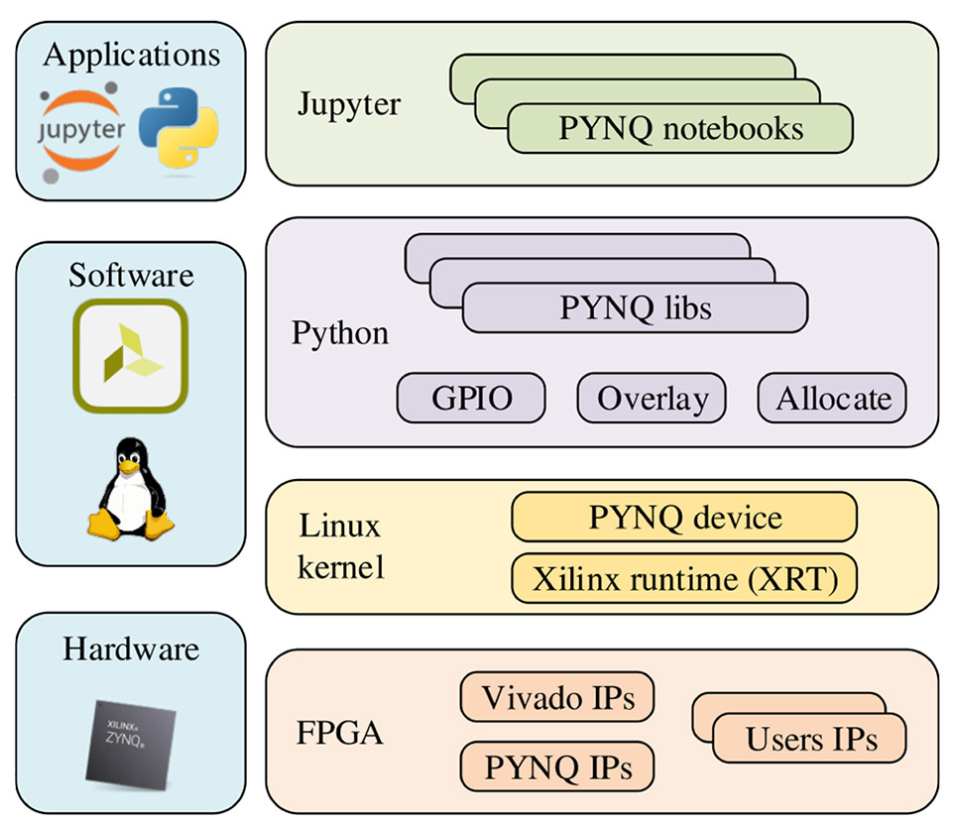
\includegraphics[width=0.42\linewidth]{obrazky-figures/firefox_8RWZKxOqlq.png}
    \caption{Celkový rámec používania PYNQ na vývoj Zynq.~\cite{LiHaoran2024AFio}}
\end{figure*}

Aplikačná vrstva je zvyčajne kód Pythonu vo forme notebooku Jupyter, ktorý beží na ARM CPU vnútri Zynq SoC. Stredná vrstva v~rámci PYNQ je softvérová. Táto vrstva obsahuje knižnice Python a~interakciu s~IP vo vnútri FPGA cez ovládače operačného systému. Niekoľko ovládačov je poskytovaných prostredníctvom knižníc PYNQ na interakciu s~IP. Rozhranie sa nazýva prekrytie (overlay) a~používa sa na programovanie FPGA a~správu IP. Poslednou hardvérovou vrstvou v~rámci PYNQ je bitový súbor naprogramovaný do FPGA, dané bitové súbory je možné vytvárať napríklad pomocou programu Vivado a~užívateľ ich môže spúšťať a~pracovať s~nimi pomocou Jupyter Notebooku, ktorý PYNQ hosťuje. Interakcia medzi softvérovou vrstvou a~hardvérovou vrstvou prebieha pomocou DMA alebo pamäťovo mapovaných rozhraní.~\cite{BjergeKim2021Asae}

\subsection{Jupyter Notebook}
Jupyter Notebook je interaktívne počítačové prostredie dostupné cez prehliadač. Je v ňom možné vytvárať dokumenty Jupyter Notebooku, ktoré obsahujú živý kód, interaktívne widgety, grafy, komentáre, rovnice, obrázky a~videá. Dosku podporujúcu nadstavbu PYNQ je možné jednoducho naprogramovať a~ovládať z~Jupyter Notebook pomocou Pythonu.

Notebook je schopný spúšťať kód v~širokej škále jazykov. Každý notebook je však spojený s~jedným jadrom. Pynq a~tento notebook je spojený s~jadrom IPython, na ktorom je spustený kód Python.
Jupyter Notebook kombinuje tri komponenty:
\begin{itemize}
    \item Webová aplikácia notebooku: Interaktívna webová aplikácia na interaktívne písanie a~spúšťanie kódu a~vytváranie dokumentov notebooku.
    \item Jadrá: Samostatné procesy spustené webovou aplikáciou notebooku, ktorá spúšťa kód používateľov v~danom jazyku a~vracia výstup späť do webovej aplikácie notebooku. Jadro tiež zvláda veci ako výpočty pre interaktívne widgety, vypĺňanie kariet a~introspekciu.
    \item Dokumenty poznámkového bloku: Samostatné dokumenty vo webovej aplikácii, ktoré obsahujú reprezentáciu celého obsahu poznámkového bloku vrátane vstupov a~výstupov výpočtov, popisného textu, rovníc, obrázkov a~multimediálnych reprezentácií objektov. Každý dokument poznámkového bloku má svoje vlastné jadro.
\end{itemize}

Používateľské rozhrania ako správa súborov, možnosti vytvorenia nového súboru a~prehlad bežiacich dokumentov poznámkového bloku sú znázornené na obrázku \ref{jupyter}.~\cite{pynqDoc}


\begin{figure*}[b] \label{jupyter}
    \centering
    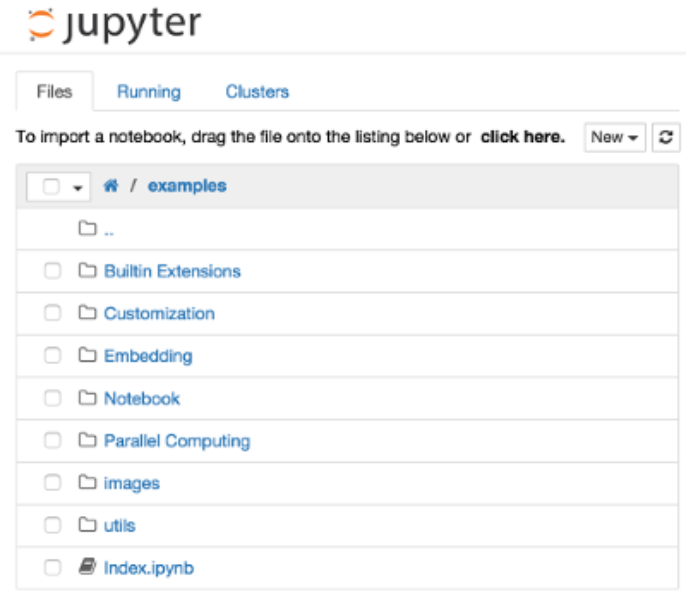
\includegraphics[width=0.35\linewidth]{obrazky-figures/firefox_cb7riywHcl.png}
    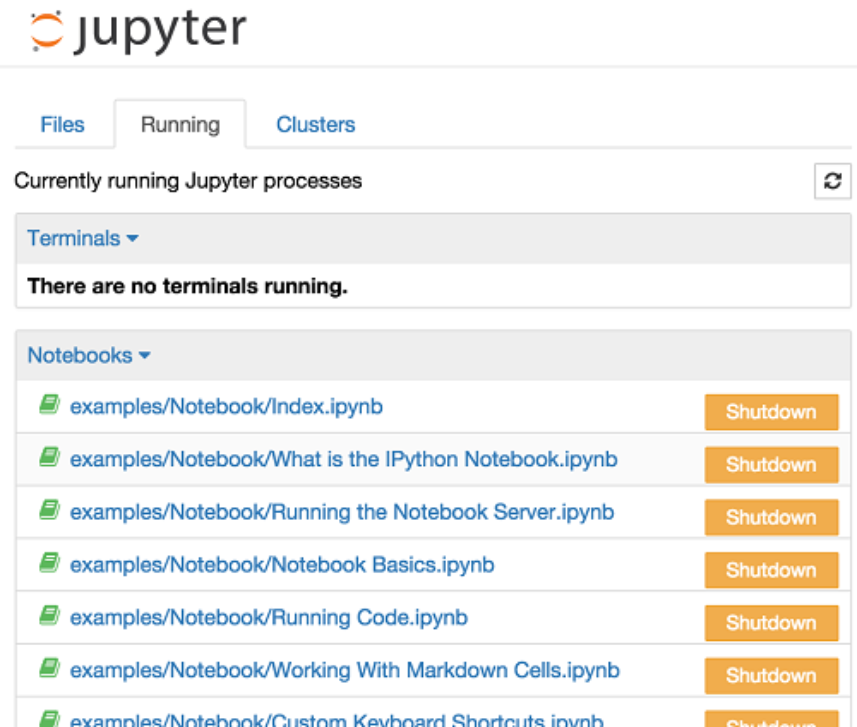
\includegraphics[width=0.35\linewidth]{obrazky-figures/firefox_9oJYQhp7gx.png}
    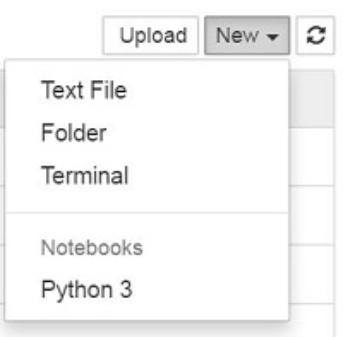
\includegraphics[width=0.2\linewidth]{obrazky-figures/firefox_n4h9S12Nm1.png}
    \caption{Používateľské rozhranie Jupyter Notebooku~\cite{pynqDoc}}
\end{figure*}


\subsection{Prístupy a~práva}
K~linux shellu sa dá dostať klasicky pomocou seriálového pripojenia, po LAN pripojení a~nastavení cez SSH klient, ale aj cez webovú aplikáciu Jupyter Notebook. Na prístup k~linuxu sa musí užívateľ verifikovať, je možné mať viacej rôznych používateľov s~rôznymi právami a~v~rôznych skupinách.

Jupyter Notebook aplikácia beží pod používateľom \verb|root|, ale je možné nastaviť, aby pri otvorení napríklad terminálu bol prihlásený dopredu zvolený používateľ. Nastaviť sa dá aj hlavný pracovný priečinok pre aplikáciu Jupyter Notebook.~\cite{pynqDoc}


\chapter{Návrh}
\label{Navrh}
V~tejto kapitole je podrobne popísaný návrh aplikácie, najprv popisujem vysoko-úrovňový diagram aplikácie a~po ňom nasleduje popis jednotlivých komponentov aplikácie. Vzhľadom k~tomu, že ide aj o~tvorbu používateľského prostredia pre študentov aj lektorov, predstavím diagram použitia. Bude tu navrhnutý databázový model pomocou ER diagramu a~v~závere sa budem venovať metodike prepojenia jednotlivých kľúčových súčastí systému.

Účelom tejto aplikácie bude poskytnúť študentom online a~časovo neobmedzený prístup ku zariadeniam, ktoré by si inak museli vypožičať od školy a~sami nastaviť.

Na základe zadania navrhujem aplikáciu, ktorá bude dostupná cez webový prehliadač, pre študenta daného predmetu, kde po prihlásení bude môcť si rezervovať časový úsek, počas ktorého bude môcť na danom zariadení pomocou hosťovaného Jupyter Notebooku spúšťať predom preložené binárne súbory z~programu Vivado. Ďalej v~tejto webovej aplikácii bude môcť, aj mimo rezervovaného časového úseku, spravovať svoje súbory, s~ktorými pracoval na registrovanom zariadení.

Na základe vypracovanej štúdie na tému zdieľania prostriedkov viacerým používateľom som sa rozhodol, že aplikáciu implementujem pomocou rezervácie jednotlivých časových úsekov, čo bude jednoduchšie a~pre účely výučby predmetu IVH vhodnejšie ako použitie plánovacích frontov. Takto bude možné každému používateľovi poskytnúť počas rezervovaného časového úseku interaktívne prostredie Jupyter Notebook, pomocou ktorého bude môcť interagovať s~rezervovaným koncovým zariadením PYNQ a~tak isto so svojimi vlastnými perifériami, ktoré si pre FPGA časť vytvoril, čo by nebolo možné pri implementácii plánovacích frontov.

K~tejto aplikácii bude mať prístup aj admin, ktorý po prihlásení sa bude môcť nahrávať nových užívateľov z~\verb|csv| súboru, spravovať rezervácie všetkých študentov a~blokovať alebo odblokovať jednotlivé PYNQ zariadenia pri poruche alebo údržbe.

Z~pohľadu bezpečnosti sa od aplikácie očakáva, aby každý používateľ mal zabezpečený prístup k~svojim dátam, ktoré mu iný používateľ nebude môcť zmeniť. Takisto aj prístup na jednotlivé koncové zariadenia PYNQ bude zabezpečený len pre daného používateľa, ktorý si vytvoril rezerváciu a~každé zariadenie bude pre tohto používateľa pripravené, a~tak nebude možné, aby mal prístup k~dátam iného používateľa.

V~aplikácii bude možné si rezervovať časový úsek najviac na jeden deň dopredu. V~rezervovanom časovom úseku sa užívateľovi objaví tlačidlo, ktorým sa mu z~jeho zariadenia vytvorí cez webový server tunel na rezervované zariadenie a~zobrazí sa mu na webovej stránke, stránka Jupyter Notebooku hosťovaného na ním rezervovanom zariadení, kde už bude môcť pracovať podľa svojich potrieb.

\section{Prípady použitia aplikácie}

V~tejto sekcii popisujem detailne každú interakciu používateľa a~aplikácie. Prípady použitia aplikácie sú dôležitou časťou návrhu aplikácie, pomáhajú s~pochopením funkčných požiadaviek systému, uľahčujú komunikáciu medzi zainteresovanými stranami a~poskytnú základ na vytváranie testovacích prípadov.

V~aplikácii budú vystupovať nasledovní používatelia: študent, admin a~čas.
\begin{itemize}
    \item Študent je klasický používateľ, ktorého úlohou v~aplikácii je vytvoriť si a~manažovať rezervácie, manažovať a~pristupovať k svojim súborom a~pristupovať k~rezervovaným zariadeniam PYNQ.
    \item Admin bude mať prístup ku všetkým funkciám ako študent, ale navyše bude mať prístup k administratívnemu rozhraniu, kde bude môcť zobrazovať a~mazať rezervácie všetkých študentov, zablokovať a~odblokovať zariadenia PYNQ podľa potreby, zobrazovať prebiehajúce pripojenia na jednotlivé zariadenia PYNQ a~nahrávať nové používateľské účty do aplikácie.
    \item Úlohou času v~aplikácii bude zobrazovanie tlačidla na prístup k~rezervovanému zariadeniu PYNQ pre jednotlivých používateľov, ak im aktuálne prebieha rezervovaný časový úsek. Po uplynutí časového úseku bude používateľ mať stále možnosť pokračovať vo svojej práci na teraz už nie rezervovanom zariadení, pokým ďalší používateľ, ktorý má toto zariadenie rezervované, nevytvorí pripojenie na toto zariadenie.
\end{itemize}

V~ďalších sekciách dopodrobna popisujem každý prípad použitia aplikácie zobrazený na obrázku diagramu použitia \ref{use case diagram}.

\subsection{Zobrazenie používateľových rezervácií}

Keďže na vytvorenie alebo zrušenie rezervácie používateľa je potrebné najprv si zobraziť svoje rezervácie, popíšem tento prípad použitia ako prvý. Používateľ bude mať prístup na stránku cez tlačidlo v~navigačnej lište, kde sa mu zobrazia všetky časové úseky na ďalší deň. Každý časový úsek bude zobrazovať informáciu, koľko zariadení je už rezervovaných z~koľkých voľných. Pre každý časový úsek bude zobrazené tlačidlo rezervovať alebo zrušiť rezerváciu podľa toho, či má študent v~danom časovom úseku vytvorenú rezerváciu. 

\subsection{Vytvorenie rezervácie}

Po kliknutí na tlačidlo rezervovať bude študentovi vytvorená rezervácia na daný vybraný časový úsek. Klientska časť kontaktuje serverovú aplikáciu, ktorá následne spraví záznam v~databáze s~používateľovým ID a~zvoleným časovým úsekom.


\subsection{Zmazanie rezervácie}

Po kliknutí na tlačidlo zrušiť rezerváciu bude študentovi zrušená rezervácia na daný vybraný časový úsek. Klientska časť kontaktuje serverovú aplikáciu, ktorá následne vymaže záznam v~databáze podľa používateľovho ID a~zvoleného časového úseku.

\subsection{Zobrazenie používateľových súborov}

Podobne ako pri práci s~rezerváciami, ak bude chcieť používateľ pracovať so~svojimi súbormi, bude si ich najprv musieť zobraziť. Po kliknutí na tlačidlo v~navigačnej lište sa používateľovi zobrazí stránka so~všetkými jeho súbormi, ktoré má uložené na serveri. Používateľovi sa najprv zobrazia všetky priečinky a~súbory v~nich, zobrazenie týchto priečinkov a~súborov bude znázorňovať strom pre lepšiu orientáciu.

\subsection{Nahrať súbory}

Používateľ bude mať možnosť nahrať súbory priamo na stránke, kde budú zobrazené všetky súbory. Na nahratie súboru bude použitý formulár, ktorý kontaktuje serverovú aplikáciu, ktorá súbor spracuje a~uloží do používateľovho priečinku.

\subsection{Stiahnuť/Zmazať súbory}

Používateľ si bude môcť každý súbor alebo priečinok stiahnuť alebo vymazať. Každý súbor/priečinok bude mať tlačidlo, vďaka ktorému si ho používateľ bude môcť stiahnuť či vymazať. Pri mazaní priečinkov aplikácia zmaže celý obsah priečinka. Pri sťahovaní priečinka aplikácia vytvorí z~vybraného priečinka \verb|zip| súbor, ktorý následne pošle používateľovi. Používateľovi bude tak isto umožnené stiahnuť/zmazať celý obsah jeho osobného priečinka na serveri.

\subsection{Pristúpiť k~rezervovanému zariadeniu}

Na pristúpenie k~rezervovanému zariadeniu si bude musieť používateľ rezervovať časový úsek; keď tento časový úsek nastane, aplikácia zobrazí používateľovi tlačidlo v~navigačnej lište. Po kliknutí na toto tlačidlo serverová aplikácia vytvorí pomocou démona spojenie medzi klientom a~zariadením PYNQ. Tak isto toto PYNQ pripraví na prácu nového používateľa, a~to tým, že reštartuje službu Jupyter Notebook, odpojí pracovný adresár predošlého používateľa a~pripojí pracovný adresár aktuálneho používateľa, následne bude používateľ presmerovaný na stránku aplikácie, kde bude už vložená hosťovaná stránka Jupyter Notebooku.

\subsection{Prihlásenie/Odhlásenie}

Používateľ sa bude môcť prihlásiť a~odhlásiť z~aplikácie pomocou prihlasovacích údajov, ktoré mu budú poskytnuté adminom aplikácie. Prihlasovacie mená a~zahašované heslá používateľov budú uložené v~databáze.

\subsection{Nahranie nových používateľov} 

Admin bude mať možnosť nahrať nových používateľov v~administračnom rozhraní. Admin nahrá \verb|csv| súbor s~používateľskými menami pomocou formulára, serverová aplikácia tieto mená spracuje, každému používateľovi vygeneruje heslo, uloží jeho prihlasovacie údaje do databázy a~následne vytvorí súbor s~používateľskými menami a~heslami, ktorý uloží do adminovho správcu súborov.

\subsection{Zobraziť rezervácie všetkých používateľov}

Admin si bude môcť v~administračnom rozhraní zobraziť rezervácie všetkých používateľov. Na stránke bude zobrazený zoznam všetkých časových úsekov na najbližší deň a~pod každým časovým úsekom bude zoznam všetkých používateľských rezervácií, každá rezervácia bude mať tlačidlo na zmazanie.

\subsection{Zrušiť rezerváciu používateľovi}

Admin bude môcť zrušiť akúkoľvek rezerváciu používateľovi pomocou tlačidla zrušiť vedľa danej rezervácie. Po stlačení tlačidla serverová aplikácia bude zavolaná a~následne rezerváciu vymaže z~databázy. Admin následne dostane notifikáciu o~úspešnom alebo neúspešnom zmazaní.

\subsection{Zablokovať/Odblokovať zariadenie}

Admin bude vidieť stav každého zariadenia PYNQ v~systéme a~bude mať možnosť toto zariadenie zablokovať alebo odblokovať podla potreby. Keď admin zariadenie zablokuje a~bude na ňom aktuálne prebiehať komunikácia medzi zariadením a~klientom, bude táto komunikácia pomocou démona zrušená a~zariadenie vyčistené. Následne zariadenie bude prepnuté do stavu ``DISABLED`` a~všetky rezervácie v~budúcnosti, ktoré by teraz prevyšovali maximálny počet zariadení, budú zrušené. Adminovi príde potvrdenie o~tom, že zariadenie bolo zablokované a~údaje o~zrušenej komunikácii a~rezerváciách sa mu uložia do správcu súborov. 

\begin{figure*} \label{use case diagram}
    \centering
    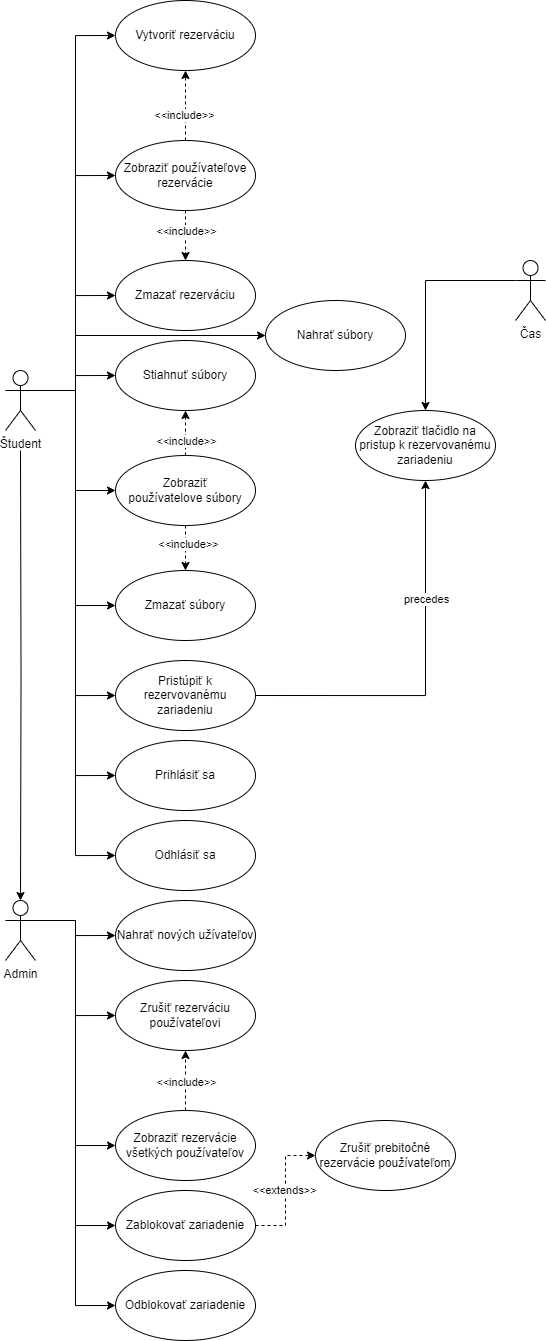
\includegraphics[width=0.55\linewidth]{obrazky-figures/Use_case_diagram.png}

    \caption{Diagram použitia}
\end{figure*}

\section{Prehľad aplikácie na vysokej úrovni}

Aplikácia virtuálne laboratórium je navrhnutá na zefektívnenie procesu výučby jazyka VHDL na zariadeniach PYNQ. Platforma bude pozostávať z~komponentov: klientske rozhranie, serverová aplikácia, databáza a~jednotlivé cieľové zariadenia PYNQ.

Prepojenie medzi týmito komponentmi je znázornené na obrázku \ref{high-level overview}. Používateľ sa bude môcť pripojiť k~webovému serveru, kde bude bežať webová aplikácia s~klientskym roz-hraním, ktoré umožní užívateľovi rezervovať si časový úsek na prácu so~zariadením PYNQ. Na serveri bude bežať démon, ktorý bude komunikovať so~serverovou aplikáciou, pomocou REST API a~na základe tejto komunikácie bude poskytovať informácie alebo vykonávať jednotlivé príkazy, ako napríklad vytvorenie tunela medzi PYNQ zariadením a~užívateľom, vyčistenie zariadenia po užívateľovi a~príprava zariadenia pre ďalšieho užívateľa.

Zariadenia PYNQ budú pripojené na lokálnej sieti s~webovým serverom, takže sa k nim užívateľ bez vytvorenia tunela nebude môcť dostať. Každé zariadenie PYNQ bude mať na jeho IP adresu a~port, na ktorom hosťuje Jupyter Notebook, priradený port na strane webového serveru v~predsmerovacej NAT tabuľke. V~posmerovacej NAT tabuľke bude na webovom serveri nastavená maškaráda na všetky zariadenia. Následne podľa potreby bude démon vytvárať pravidlá v~presmerovacej tabuľke pre jednotlivých používateľov, ktorí majú aktuálne prebiehajúci registrovaný časový úsek.

Webový server bude komunikovať aj s~jednoduchou databázou, ktorá bude slúžiť na ukladanie prihlasovacích údajov používateľov a~jednotlivých registrácií časových úsekov používateľov.

\begin{figure*}[t] \label{high-level overview}
    \centering
    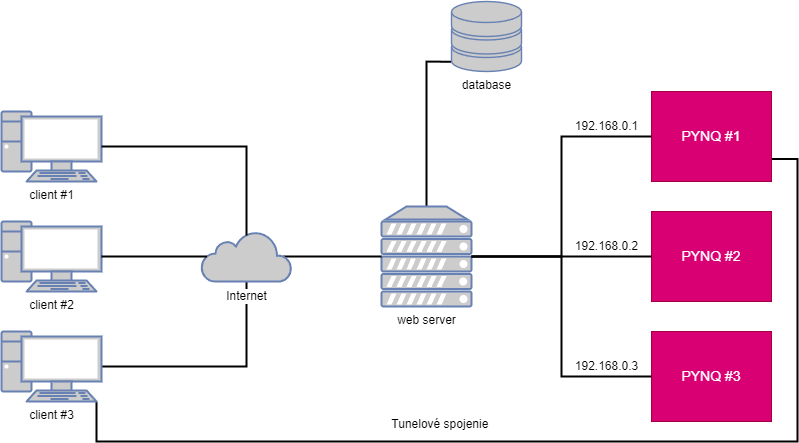
\includegraphics[width=1\linewidth]{obrazky-figures/High_Level_diagram.png}
    \caption{Prehľad na vysokej úrovni}
\end{figure*}

\section{Komponenty aplikácie}

Aplikácia bude pozostávať z~troch hlavných komponentov: klientske rozhranie, serverové rozhranie a~jednotlivé zariadenia PYNQ.

\subsection{Klientske rozhranie}

Klientske rozhranie, kam budú mať používatelia prístup, umožní používateľom registrovať si jednotlivé časové úseky pre prácu na zariadeniach PYNQ. Tak isto aj spravovať svoje registrácie. Pomocou tohto rozhrania im bude umožnená práca na jednotlivých koncových zariadeniach PYNQ pomocou vloženia hosťovanej Jupyter Notebook web stránky z~registrovaného zariadenia PYNQ na hlavnú stránku webovej aplikácie. Pomocou tejto Jupyter Notebook stránky bude užívateľ nahrávať a~spúšťať pred-kompilované binárne súbory, vytvárať Jupyter Notebook dokumenty, môcť ovládať zariadenie pomocou spomínaných Jupyter Notebook dokumentov použitím programovacieho jazyka Python, alebo dokonca spustiť si terminál s~Linux shell prostredím a~spúšťať príkazy priamo tam.

Klientske rozhranie umožní používateľom spravovať svoje pracovné súbory aj mimo registrovaný časový úsek, a~to pomocou súborového manažéra, ktorý umožní používateľom mazať, nahrávať a~sťahovať súbory, ktoré budú dostupné aj na zaregistrovanom zariadení PYNQ.

Klientske rozhranie používateľom neumožní vytvoriť si účet, a~to kvôli bezpečnosti. Používateľské účty bude môcť vytvárať iba admin tejto aplikácie, ktorý v~aplikácii v~administračnom rozhraní nahrá \verb|csv| súbor s~používateľskými menami a~serverová aplikácia, každému používateľovi vygeneruje náhodne heslo a~vytvorí mu účet. Admin potom vo svojom súborovom manažéri v~aplikácii bude mať \verb|csv| súbor, ktorý bude obsahovať používateľské mená s~vygenerovanými heslami a~vlajkou úspechu vytvorenia používateľského účtu pre každého používateľa.

Admin si tak isto bude môcť zobraziť všetky rezervácie používateľov a~ak bude niekto schválne blokovať ostatných užívateľov, tak mu tieto rezervácie bude môcť zrušiť. Admin uvidí stav každého zariadenia PYNQ. Ak k~nemu v~danom momente bude mať niekto vytvorený tunel, admin uvidí podrobnosti tohto tunela, ako je IP adresa používateľa, jeho používateľské meno a~ID v~databáze. Admin bude môcť tieto zariadenia spravovať tak, že každé z~nich bude môcť zablokovať alebo odblokovať podľa potreby, bez nutnosti zastavenia celej aplikácie, ak napríklad nastane porucha na niektorom zo zariadení, alebo sa bude jednať len o~údržbu.

\subsection{Serverové rozhranie}

Serverová aplikácia sa postará o~celú obchodnú logiku aplikácie, ako vytváranie rezervácií, autentifikácia používateľov, komunikácia s~databázou, komunikácia s~démonom, pomocou ktorého bude spravovať všetky zariadenia PYNQ, vytvárať a~odstraňovať pravidlá v~smerovacích tabuľkách, pre pripojenie používateľa k~jednotlivým zariadeniam PYNQ. Databáza bude ukladať všetky rezervácie používateľov a~prihlasovacie dáta používateľov. 

Démon bude spravovať zariadenia PYNQ pomocou SSH klienta a~upravovať pravidlá IP tabuliek. Ďalej bude komunikovať so serverovou aplikáciou pomocou REST API endpointu. Serverová aplikácia bude pomocou démona spravovať všetky pravidlá v~IP tabuľkách tak, aby na každé zariadenie PYNQ mal prístup len jeden používateľ, ktorý si to zariadenie registroval na daný časový úsek. Na spravovanie týchto pravidiel v~IP tabuľkách bude démon vytvárať smerovacie pravidlá, čím sa zaistí presmerovanie komunikácie pomocou tunela cez hosťovské zariadenie medzi zariadením PYNQ a~používateľom.

\subsection{PYNQ zariadenia}

Posledným komponentom aplikácie sú zariadenia PYNQ, ktoré budú slúžiť na spúšťanie dopredu skompilovaných binárnych súborov. Binárne súbory si používateľ dopredu naprogramuje v~ním preferovanom prostredí, väčšinou to je program Vivado. Binárne súbory si používateľ bude môcť nahrať na server aj predtým, ako sa aktivuje jeho rezervovaný časový úsek. Tieto súbory, ktoré používateľ nahrá na server, sa mu automaticky sprístupnia na ním rezervovanom zariadení. V~rezervovanom časovom úseku bude mať používateľ prístup priamo na stránke aplikácie k~Jupyter Notebooku, ktorý je hosťovaný ním rezervovaným zariadením. Vďaka tomuto Jupyter Notebooku bude môcť na zariadení spúšťať a~testovať svoje binárne súbory, vytvárať alebo nahrávať nové súbory, spúšťať Jupyter Notebook dokumenty, alebo dokonca pristúpiť k~terminálu daného zariadenia, odkiaľ bude môcť vykonávať rôzne príkazy podla svojej potreby.


\section{Diagram vzťahu entít (ER)}

V~tejto sekcii budem popisovať diagram vzťahu entít, ktorý je zobrazený na obrázku \ref{ER diagram}
Táto aplikácia bude potrebovať len dve entity, ktoré budú musieť byť uložené v~databáze: rezervácie a~používateľov.

\begin{itemize}
    \item Rezervácia: Obsahuje informácie o~rezervácii vykonanej používateľom pre daný časový úsek, ktorý bude uložený ako atribút tejto entity. Táto entita bude mať tri atribúty. Atribút \verb|res_id|, ktorý predstavuje identifikátor a~hlavný kľúč tejto entity. Atribút \verb|user_id| je cudzí kľúč z~entity user a~odkazuje na používateľa, ktorý túto rezerváciu vytvoril. Posledný atribút je \verb|time|, ktorý predstavuje časový úsek, na ktorý bola táto rezervácia vytvorená a~je uložený v~podobe časovej značky.
    \item Používatelia: Obsahuje prihlasovacie údaje používateľov a~bude pozostávať z~troch atribútov. Atribút \verb|id| bude predstavovať identifikátor používateľa v~databáze a~je primárnym kľúčom tejto entity, tento atribút bude tiež cudzím kľúčom v~entite rezervácia. Atribút \verb|username| je prihlasovacie meno používateľa a~zároveň bude unikátnym indexom v~databáze, aby sa zamedzilo používateľom s~rovnakým prihlasovacím menom. Posledným atribútom bude \verb|password|, ktorý bude predstavovať zahašované heslo používateľa.
    \item PYNQ: Každé zariadenie PYNQ bude v~systéme figurovať ako entita, ktorá bude uložená v~pamäti démona. Tieto zariadenia si démon načíta z~konfiguračného \verb|json| súboru pri spustení. Počet možných rezervácií na každý časový úsek sa bude odvíjať od počtu dostupných PYNQ zariadení. Rezervácia nebude viazaná na žiadne konkrétne zariadenie; keď nastane používateľov rezervovaný časový úsek, aplikácia vyberie jedno z~dostupných zariadení PYNQ, na ktorom aktuálne neprebieha rezervovaný časový úsek iného používateľa. Primárnym kľúčom bude IP adresa zariadenia, pod ktorou je zariadenie pripojené do súkromnej siete so serverovou aplikáciou. Atribút port bude ukladať informáciu o~tom, na ktorom porte na zariadení, kde beží serverová aplikácia, je namapovaná IP adresa zariadenia PYNQ, a~port, kde zariadenie PYNQ hosťuje webovú stránku Jupyter Notebooku. Posledný atribút bude predstavovať stav zariadenia PYNQ.  
    \item Tunel: Ide o relačnú entitu medzi používateľom a~ním aktuálne rezervovaným zariadením PYNQ. Táto entita bude predstavovať informácie o~vytvorenom tuneli z~používateľovho zariadenia na zariadenie PYNQ. Táto entita bude uložená v~pamäti démona. Tunel bude mať dva cudzie kľúče, a~to IP adresu zariadenia PYNQ, na ktorú je vytvorený, a~ID používateľa, ktorý ma dané zariadenie rezervované. Ďalej bude ukladať informáciu o~IP adrese používateľovho zariadenia, z~ktorého komunikuje so zariadením PYNQ. Atribút port znovu bude ukladať informáciu o~tom, na ktorom porte je namapovaná IP adresa a~port zariadenia PYNQ na ktorej bude dostupná hosťovaná stránka Jupyter Notebooku na zariadení, na ktorom bude bežať serverová aplikácia. 
\end{itemize}

\begin{figure*}[t] \label{ER diagram}
    \centering
    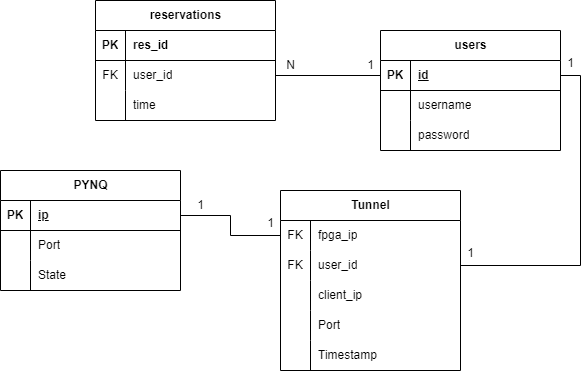
\includegraphics[width=0.8\linewidth]{obrazky-figures/ER.png}
    \caption{Diagram vzťahu entít}
\end{figure*}

\section{Prepojenie medzi komponentmi}

Pre správne fungovanie aplikácie budú musieť komponenty medzi sebou komunikovať. Na túto komunikáciu budú využité rôzne technológie, ktoré sú dostupné v~jednotlivých častiach aplikácie.

Klientske rozhranie bude komunikovať so serverovou aplikáciou pomocou volania API endpointov serverovej aplikácie, ktoré mu buď rovno odovzdajú informácie, alebo klientske rozhranie pomocou týchto endpointov pošle metódou POST dáta serverovej aplikácii.

Serverová aplikácia bude, ako už som popisoval, komunikovať s~klientskym rozhraním pomocou API endpointov a~taktiež bude komunikovať s~démonom pomocou jeho REST API endpointu, a~takisto od neho bude získavať buď informácie, alebo mu ich posielať metódou POST a~vo formáte json.

Démon bude komunikovať so serverovou aplikáciou a~aj s~jednotlivými zariadeniami PYNQ, a~to pomocou pripojenia cez SSH klienta, ktorým bude pod používateľom root spúšťať skripty na vyčistenie a~pripravenie zariadenia pre ďalšieho používateľa.

Zariadenia PYNQ budú komunikovať s~klientskym rozhraním pomocou vloženej Jupyter Notebook stránky, ku ktorej bude mať používateľ umožnený prístup pomocou vytvoreného tunela.


\chapter{Implementácia} 
\label{Implementacia}

Táto kapitola sa venuje implementácii aplikácie, pričom detailne popisuje použité technológie a~postupy, ktoré boli nevyhnutné pre vývoj aplikácie.

\section{Architektúra}

Sekcia sa venuje architektúre aplikácie, ktorá je znázornená na blokovej schéme v~obrázku \ref{Blokova schema}. Aplikácia sa skladá z~troch hlavných častí: klientskej časti, serverovej časti a~jednotlivých koncových zariadení PYNQ.

Klientska časť obsahuje používateľské rozhranie, ktoré je implementované v~jazykoch HTML, CSS a~JavaScript. Táto časť komunikuje so serverovou časťou pomocou protokolov HTTP a~HTTPS, pričom reaguje na rôzne požiadavky používateľa – buď zobrazuje webové stránky aplikácie, alebo odosiela žiadosti serverovej časti na vykonanie akcií. Klientska časť tiež komunikuje so zariadeniami PYNQ prostredníctvom protokolov HTTP a~HTTPS. Komunikácia prebieha cez vložený Jupyter Notebook, ktorý je prístupný vytvorením tunela z~používateľovho zariadenia na zariadenie PYNQ cez webový server.

Serverová časť pozostáva z~webového servera Apache, v~ktorom beží aplikácia napísaná v~jazyku PHP a~rámca Nette, z~databázy MariaDB a~z~démona. Táto časť aplikácie obsluhuje požiadavky pomocou REST API. Na základe požiadavky môže zobraziť webovú stránku, poslať dáta vo formáte json, alebo spracovať požiadavku na vykonanie určitej akcie. Démon bežiaci na serveri je napísaný v~jazyku Go a~komunikuje so serverovou aplikáciou cez REST API. Serverová aplikácia môže cez toto API poslať požiadavku na získanie dát o~zariadeniach PYNQ, tuneloch, alebo na zmenu stavu zariadenia PYNQ.

Každé zariadenie PYNQ hosťuje webovú stránku s~Jupyter Notebookom, ktorá umožňuje používateľovi ovládať zariadenie alebo spúšťať preložené súbory.


\begin{figure*}[t] \label{Blokova schema}
    \centering
    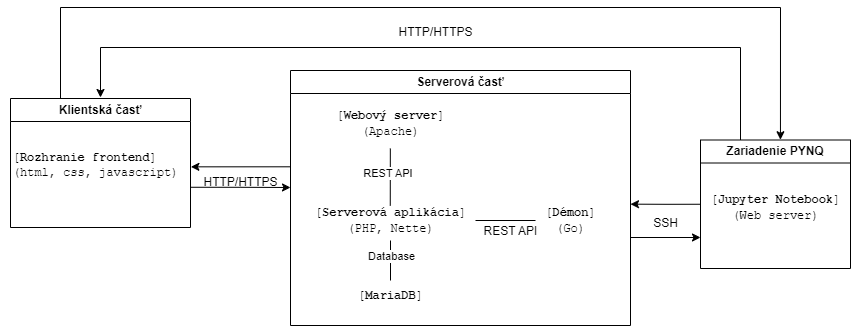
\includegraphics[width=1\linewidth]{obrazky-figures/block_diagram_architecture.png}
    \caption{Bloková schéma architektúry}
\end{figure*}

\section{Používateľské rozhranie}


Cieľom používateľského rozhrania je umožniť jednoduchú a~efektívnu interakciu používateľa s~aplikáciou. Rozhranie, napísané v~HTML, CSS a~JavaScript, je navrhnuté tak, aby bolo intuitívne a~prístupné z~akéhokoľvek zariadenia.

Rozhranie obsahuje navigačnú lištu, ktorá je konzistentne prítomná na vrchu každej stránky. Táto lišta umožňuje používateľom rýchlo prechádzať medzi rôznymi časťami aplikácie a~poskytuje informácie o~stave prihlásenia.

\subsection{Prihlasovacie rozhranie}

Prihlasovacie rozhranie, zobrazené na obrázku \ref{login page}, umožňuje používateľom zadávať svoje prihlasovacie údaje prostredníctvom formulára, ktorý sa postará o~komunikáciu so serverovou časťou aplikácie. Táto stránka je prvým bodom interakcie používateľa s~aplikáciou, zabezpečujúc tak prístup do systému.


\begin{figure*} \label{login page}
    \centering
    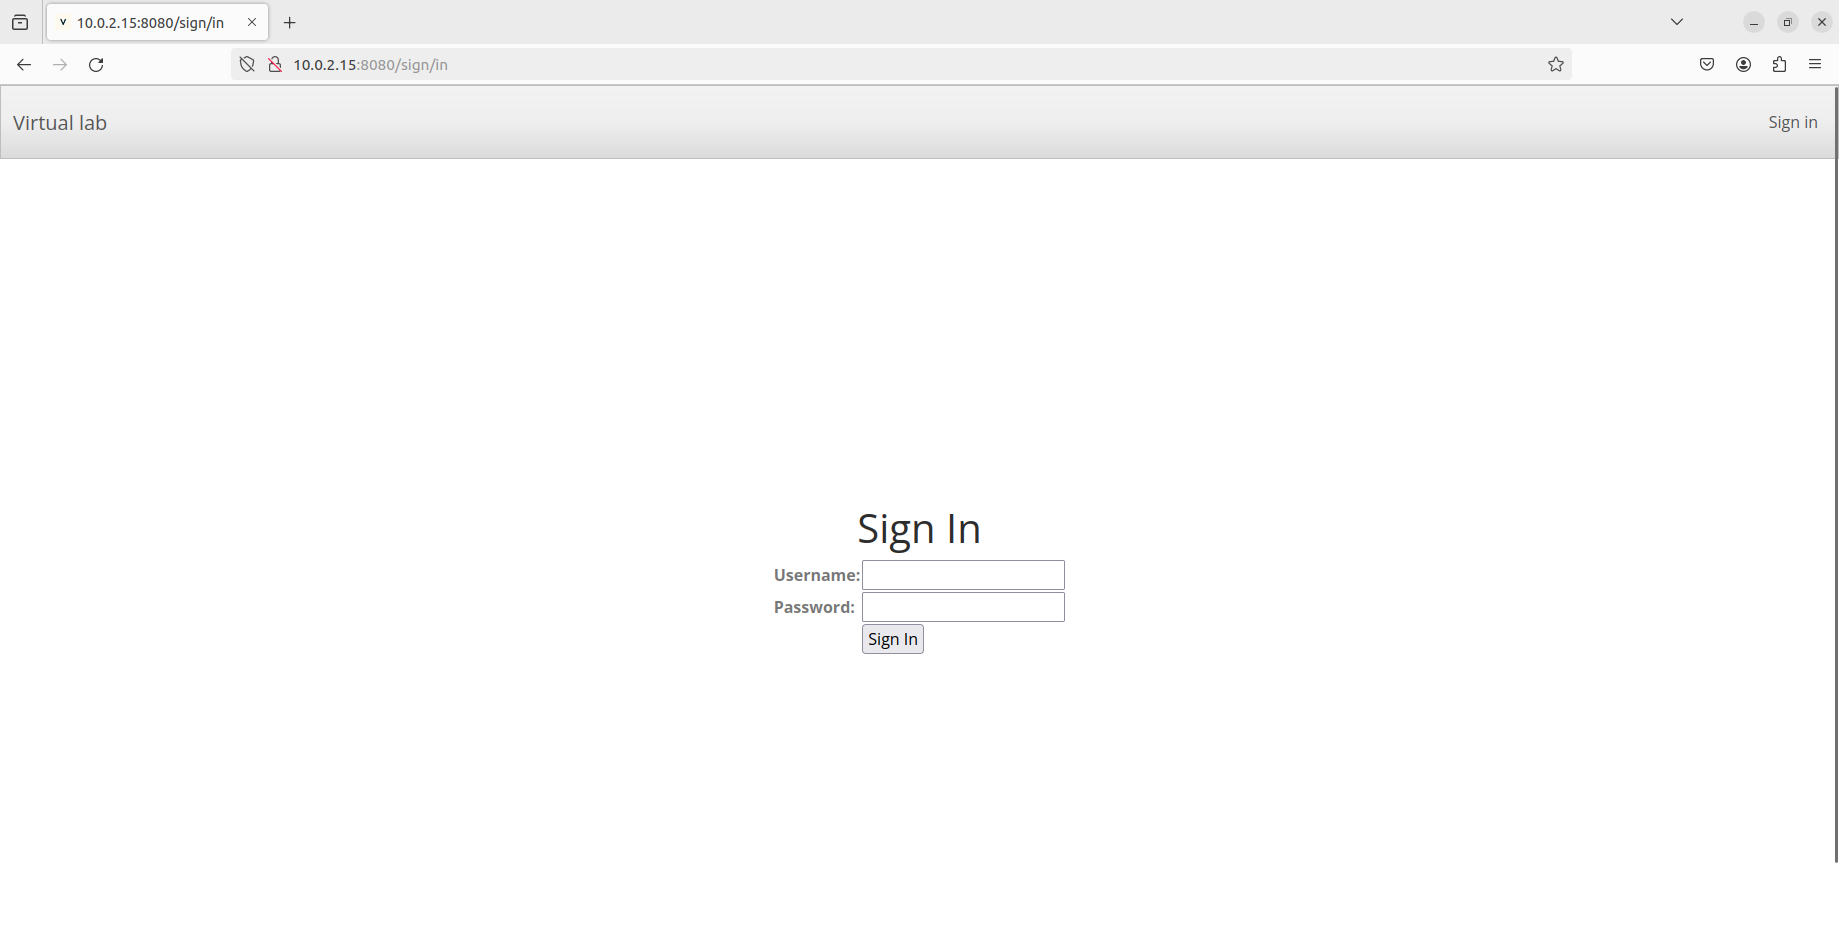
\includegraphics[width=1\linewidth]{obrazky-figures/Sign_in_site.png}
    \caption{Stránka prihlásenia}
\end{figure*}

\subsection{Uvítacie rozhranie}


Po prihlásení sa používateľ dostáva do uvítacieho rozhrania zobrazeného na obrázku \ref{Uvitacia obrazovka}, ktoré poskytne základné informácie používateľovi a~nasmeruje ho k~ďalšej interakcii s~aplikáciou. 


\begin{figure*} \label{Uvitacia obrazovka}
    \centering
    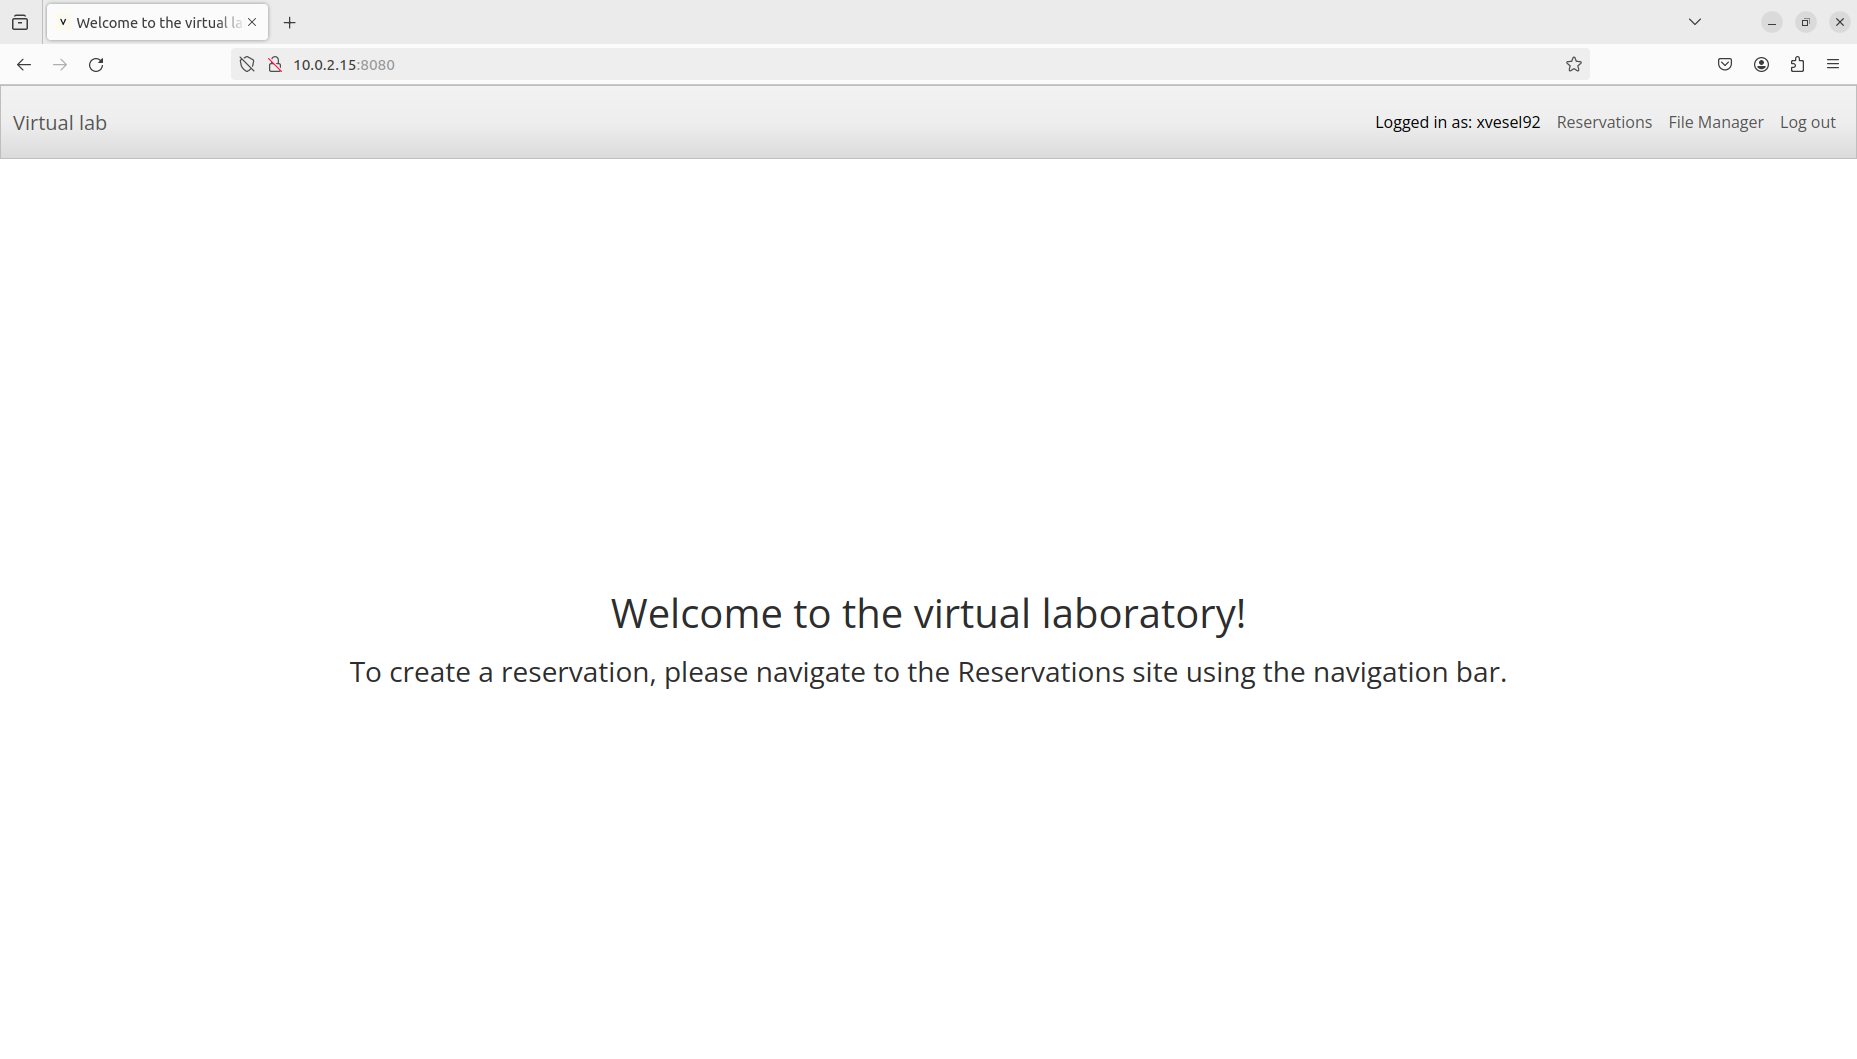
\includegraphics[width=1\linewidth]{obrazky-figures/Welcome_site.png}
    \caption{Uvítacia stránka}
\end{figure*}

\subsection{Rezervačné rozhranie}

V~rezervačnom rozhraní, ktoré je zobrazené na obrázku \ref{Rezervacna obrazovka}, si môžu používatelia rezervovať alebo odrezervovať časové úseky podľa aktuálnej dostupnosti. Táto stránka dynamicky zobrazuje dostupné časové úseky a~ich stav na základe aktuálnej dopytovej situácie. Tak isto dynamicky zobrazuje aj počet aktuálnych rezervácií prihláseného používateľa. 


\begin{figure*} \label{Rezervacna obrazovka}
    \centering
    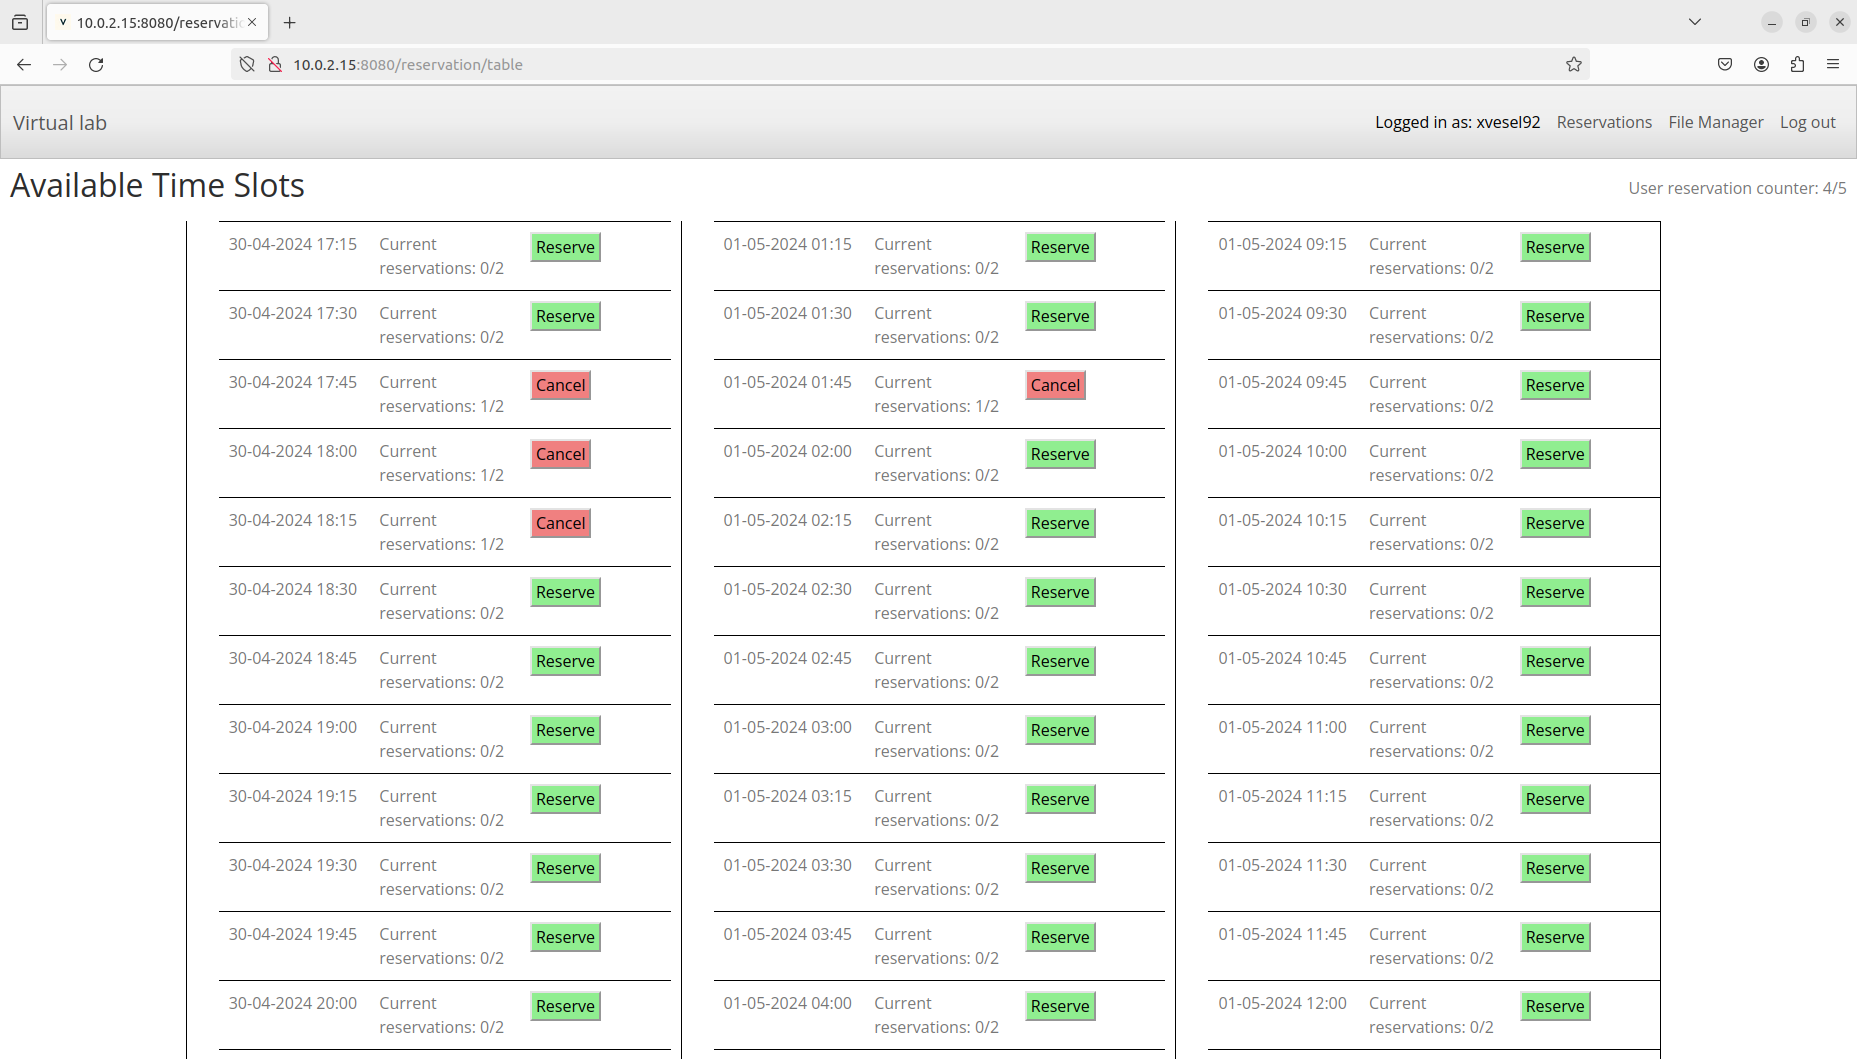
\includegraphics[width=1\linewidth]{obrazky-figures/Reservations_site.png}
    \caption{Stránka pre rezervácie časových úsekov}
\end{figure*}

\subsection{Rozhranie na správu súborov}

Rozhranie na správu súborov, zobrazené na obrázku \ref{Filemanager}, umožňuje používateľom nahrávať a~spravovať súbory v~ich osobnom pracovnom priečinku na serveri. Používatelia môžu súbory jednoducho sťahovať alebo odstraňovať a~majú tak prístup k~organizácii svojich dát v~hierarchickej štruktúre aj mimo rezervovaného časového úseku.

\begin{figure*} \label{Filemanager}
    \centering
    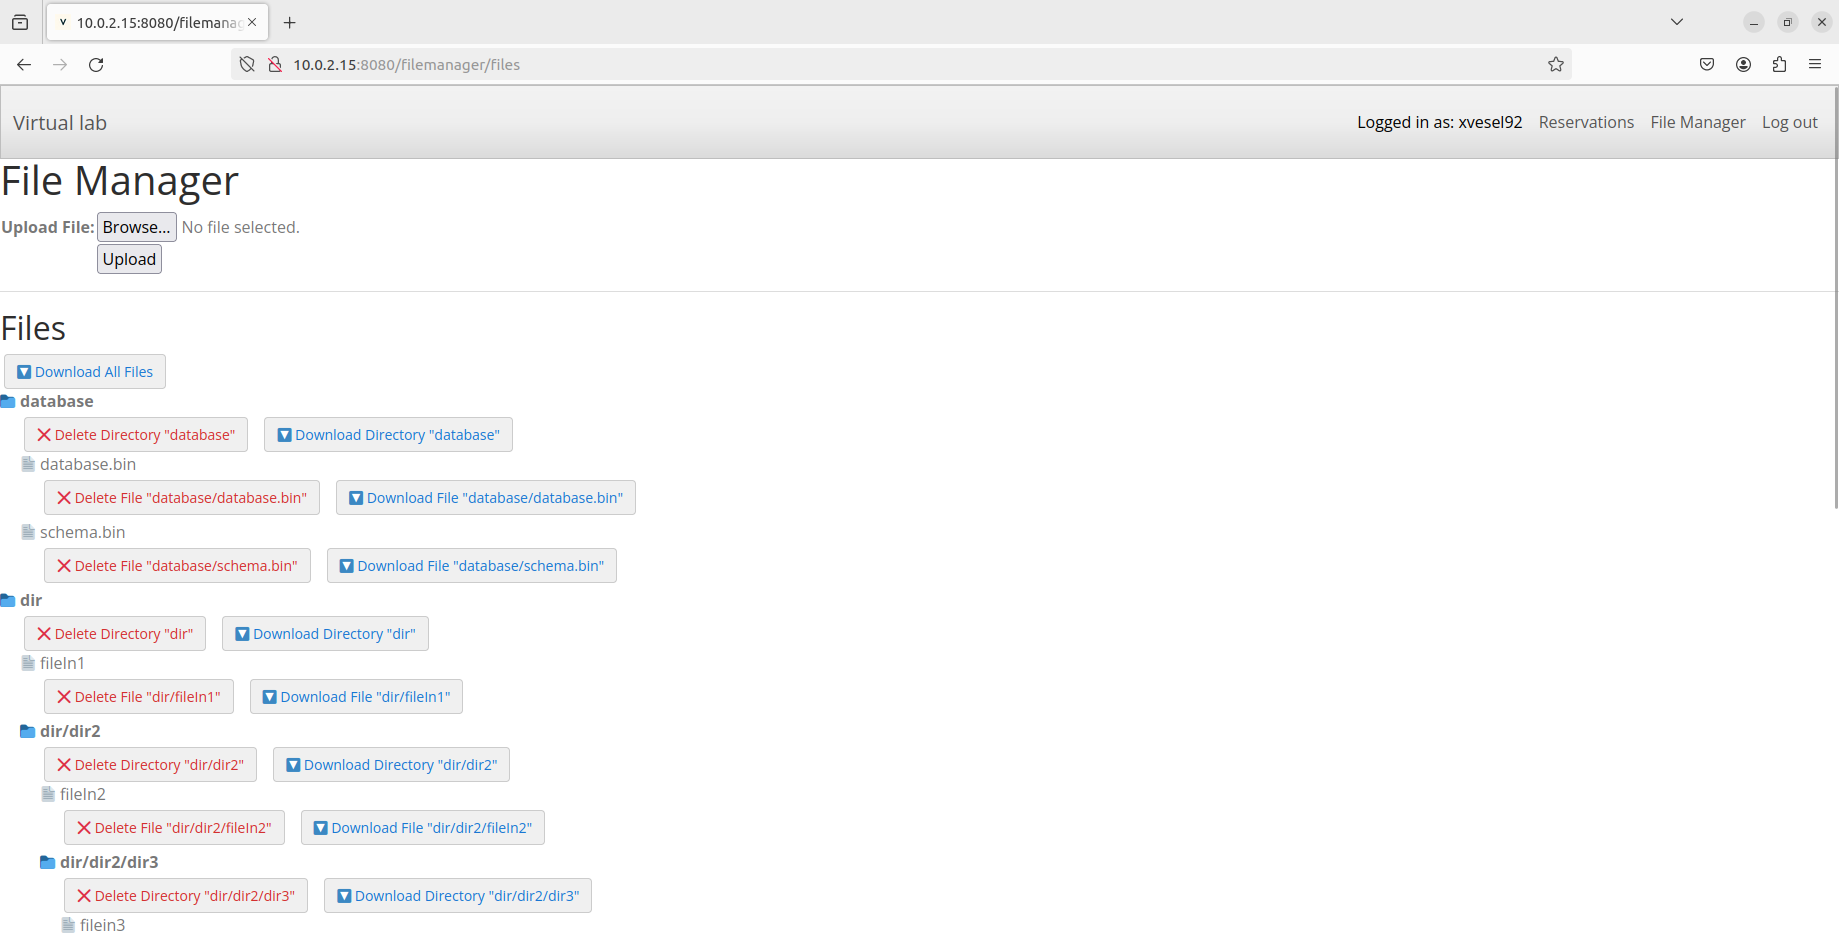
\includegraphics[width=1\linewidth]{obrazky-figures/Filemanager_site.png}
    \caption{Stránka správcu súborov}
\end{figure*}

\subsection{Rozhranie aktívneho pripojenia}

\begin{figure*} \label{Active connection}
    \centering
    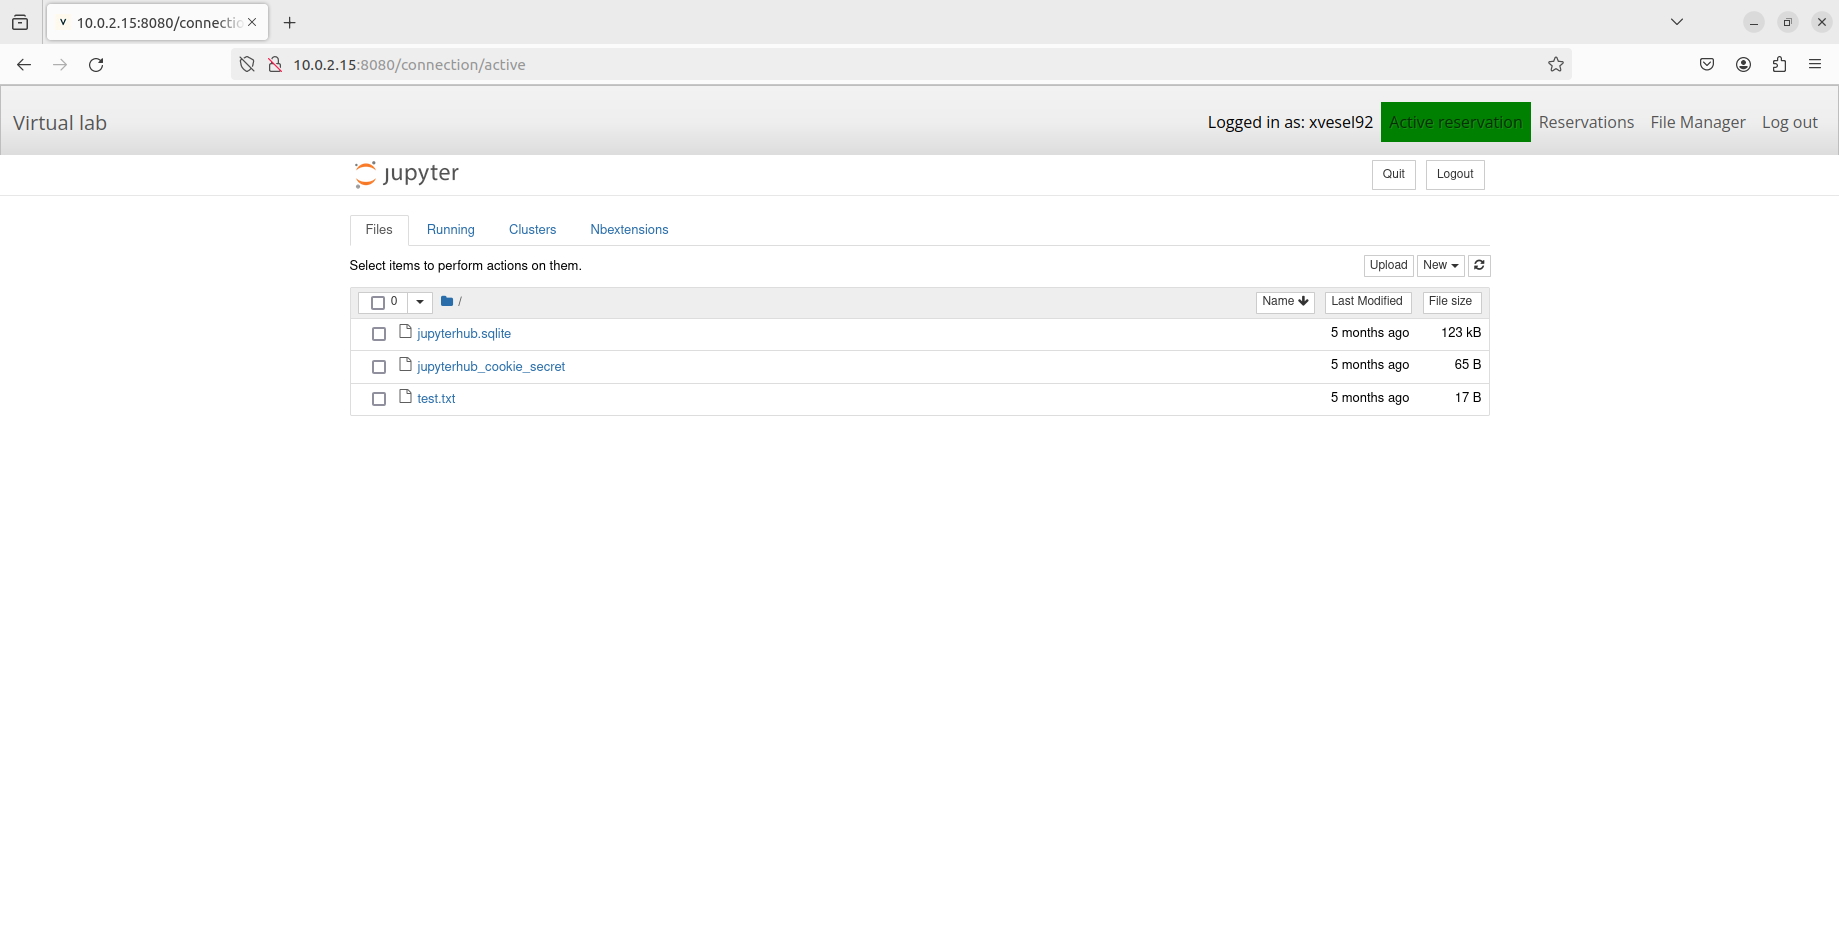
\includegraphics[width=1\linewidth]{obrazky-figures/Active_connection_site.png}
    \caption{Stránka pripojenia k~zariadeniu}
\end{figure*}

Rozhranie aktívneho pripojenia k~zariadeniu, zobrazené na obrázku \ref{Active connection}, umožňuje používateľom interagovať priamo so zariadením PYNQ cez integrovaný Jupyter Notebook. Táto stránka je dostupná iba vtedy, ak má používateľ aktívnu rezerváciu alebo vytvorené tunelové spojenie na jedno zo zariadení PYNQ.


\subsection{Administračné rozhranie}

\begin{figure*} \label{Admin panel}
    \centering
    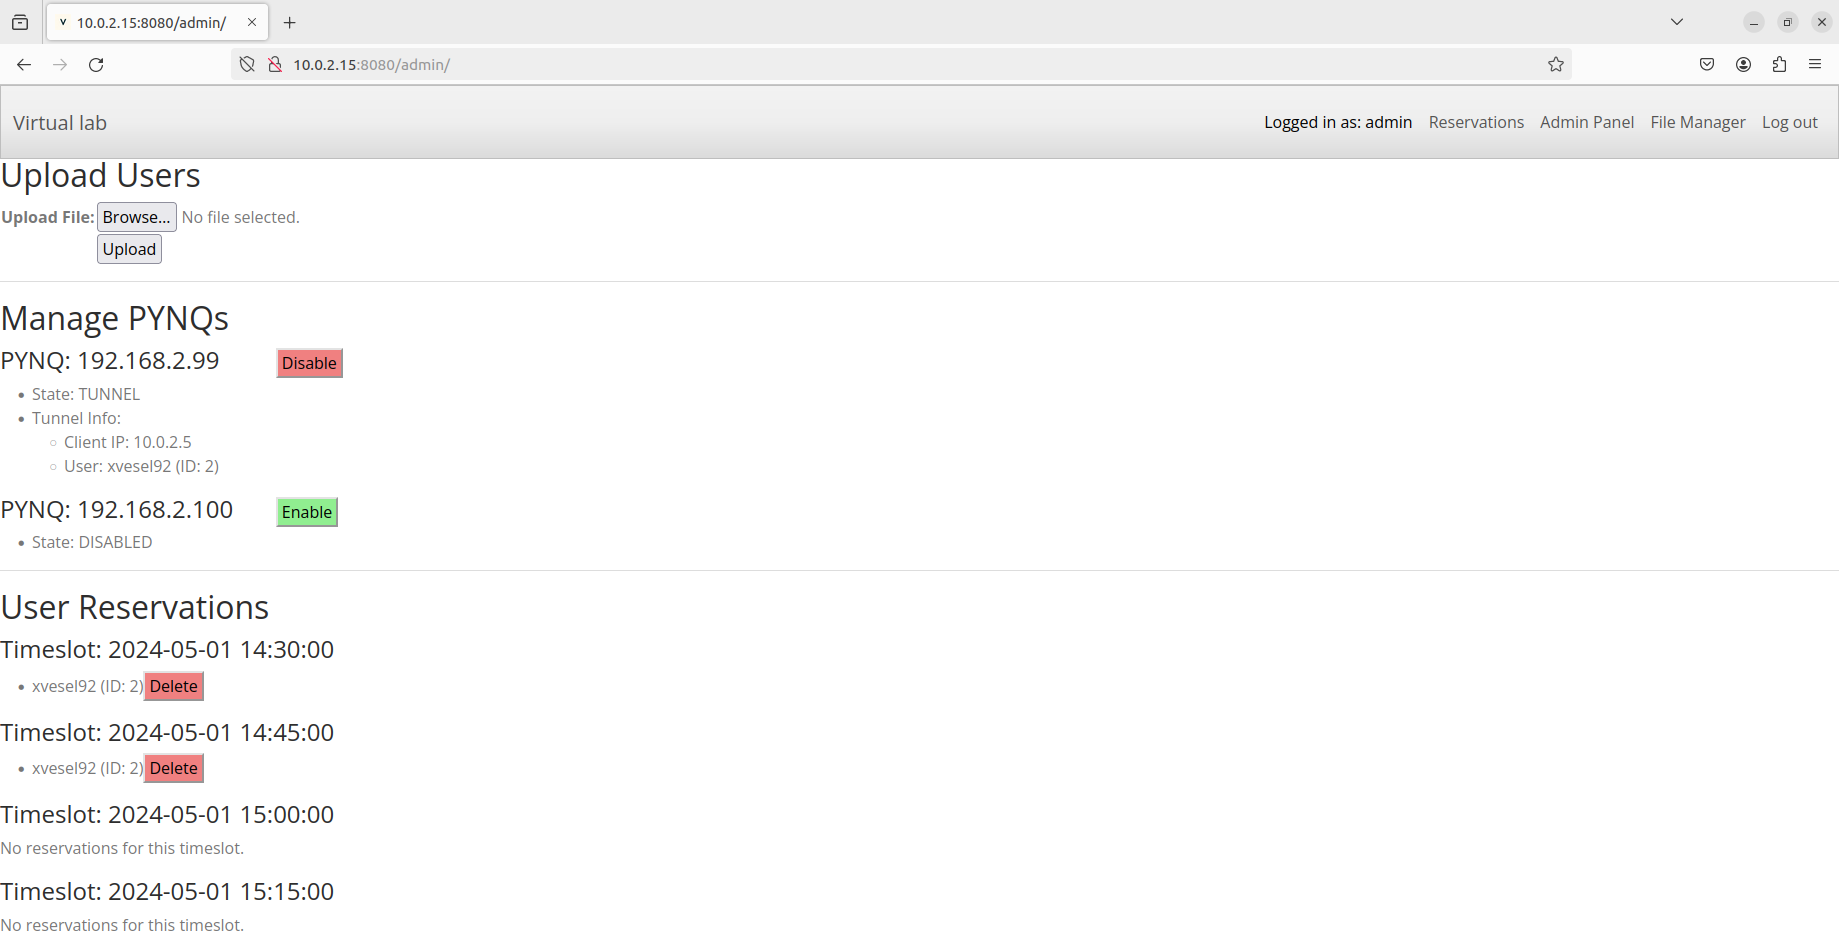
\includegraphics[width=1\linewidth]{obrazky-figures/Admin_panel_site.png}
    \caption{Stránka admin panelu}
\end{figure*}

Administračné rozhranie, zobrazené na obrázku \ref{Admin panel}, poskytuje administrátorom nástroje na správu používateľov a~jednotlivých zariadení PYNQ. Administrátori môžu pridávať nových používateľov, spravovať rezervácie časových úsekov a~monitorovať a~meniť stav jednotlivých zariadení PYNQ.


\section{Serverová aplikácia}

Serverová aplikácia zodpovedá za spracovanie požiadaviek od používateľov a~poskytuje dáta používateľskému rozhraniu. Je implementovaná v~jazyku PHP s~využitím rámca Nette, ktorý uprednostňuje architektúru založenú na prezentéroch namiesto tradičného modelu \verb|MVC|.

Rámec Nette je v~serverovej aplikácii využitý pre svoju robustnosť a~schopnosť efektívne spracovať viaceré typy požiadaviek cez REST API. Prezentéry v~Nette môže obsluhovať viaceré používateľské rozhrania a~poskytovať rôzne endpointy pre operácie ako sú zápis do databázy alebo autentifikáciu používateľov.

\subsection{Moduly a~služby serverovej aplikácie}

Pre správne fungovanie aplikácie je potrebné, aby aplikácia mohla komunikovať s~databázou, rozhraním pre správu a~komunikáciu s~PYNQ jednotkami, alebo mohla verifikovať a~spravovať používateľov či manipulovať so súbormi na serveri, toto jej umožňujú moduly, ktoré následne používajú jednotlivé prezentéry. 

\subsubsection*{ApiService a~ApiFacade}

Služba \verb|ApiService| zabezpečuje komunikáciu s~rozhraním pre správu a~komunikáciu s~jednotkami PYNQ, vrátane získavania dát o~aktívnych tuneloch a~zariadenia PYNQ, a~to pomocou REST API. V~prezentéroch je už dostupný modul \verb|ApiFacade|, ktorý umožňuje volanie týchto funkcií.

\subsubsection*{ReservationFacade}

Modul \verb|ReservationFacade| sa používa na prácu s~databázou, pomocou ktorého prezentér môže získavať, vkladať alebo mazať informácie o~rezerváciách alebo používateľoch. Tento modul umožňuje efektívne spracovanie dát spojených s~používateľskými rezerváciami.

\subsubsection*{Authenticator a~FileManager}

Modul \verb|Authenticator| sa stará o~autentifikáciu používateľov, ich verifikáciu a~správu používateľských rolí. \verb|FileManager| je použitý na manipuláciu so súbormi v~používateľských pracovných priečinkoch, čo zahŕňa vypísanie, nahrávanie, sťahovanie a~mazanie súborov.

\subsection{Funkcionalita}

Funkcionalita serverovej aplikácie je úzko spätá s~prezentérmi, ktoré komunikujú s~používateľským rozhraním, ale aj s~ostatnými komponentami v~serverovom rozhraní a~to pomocou vyššie popísaných modulov. Preto táto sekcia popisuje funkcionalitu každého prezentéru a~tým aj funkcionalitu serverovej aplikácie.

\subsubsection*{DefaultPresenter}

\verb|DefaultPresenter| v~rámci serverovej aplikácie plní kľúčovú úlohu v~riadení prístupu a~poskytovaní dát používateľom. Hlavnými funkcionalitami prezetéra sú autentifikácia a~poskytnutie mena aktuálne prihláseného používateľa do navigačnej lišty. Pri každom volaní prezentér zabezpečuje kontrolu, či je používateľ prihlásený. Ak nie je prihlásený, automaticky ho presmeruje na prihlasovaciu stránku. Ak je používateľ prihlásený, jeho meno je poslané do šablóny, ktorá sa používa na zobrazenie navigačnej lišty, čo umožňuje aplikácii personalizovať užívateľské rozhranie. Prezentér poskytuje aj niekoľko endpointov: 

\begin{itemize}
    \item \verb|get-live-reservation|: Zistí, či má používateľ aktuálne prebiehajúcu rezerváciu zariadenia, alebo aktívne tunelové spojenie na zariadenie PYNQ. Tento endpoint je dôležitý pre dynamické zobrazenie tlačidla na prístup do rozhrania aktívneho pripojenia.
    \item \verb|buttons|: Endpoint generuje \verb|JSON| odpoveď s~dátami pre jednotlivé tlačidlá, ktoré reprezentujú časové úseky.
    \item \verb|allreservations|: Poskytuje počet všetkých rezervácií pre každý časový úsek v~systéme, čo umožňuje používateľom získať prehľad o~obsadenosti jednotlivých časových úsekov.
    \item \verb|get-fpga-count|: Vracia počet všetkých dostupných zariadení PYNQ v~systéme.
    \item \verb|get-user-reservation-count|: Informuje o~celkovom počte rezervácií, ktoré má aktuálne prihlásený používateľ.
    \item \verb|reservation|: Tento endpoint umožňuje vytvorenie alebo zrušenie rezervácie na základe poskytnutých údajov cez POST metódu. Endpoint skontroluje, či je rezervácia možná bez prekročenia kapacitných limitov a~vykoná požadovanú akciu, či už pridanie alebo odstránenie rezervácie.
    
\end{itemize}

\subsubsection*{LandingPagePresenter}

\verb|LandingPagePresenter| v~serverovej aplikácii plní jedinú úlohu, a~to je vykreslenie uvítacej stránky aplikácie, ktorej poskytuje statickú správu do šablóny, ktorá je následne vykreslená.

\subsubsection*{ReservationPresenter}

\verb|ReservationPresenter| je prezentér ktorý v~rámci serverovej aplikácie zohráva významnú rolu pri správe a~zobrazení časových úsekov na rezerváciu. Jeho primárnou funkciou je zobraziť používateľom dostupné časové úseky na rezerváciu v~prehľadnej a~organizovanej forme. 

Prezentér generuje časové úseky v~15-minútových intervaloch na nasledujúci deň. Tieto časové úseky distribuuje do troch stĺpcov, čím uľahčí vizuálnu orientáciu a~tým pomáha používateľom rýchlo identifikovať dostupné časové úseky.

\subsubsection*{SignPresenter}

\verb|SignPresenter| je zodpovedný za spracovanie prihlásenia do aplikácie. Jeho hlavnou úlohou je zobraziť a~spracovať prihlasovací formulár, čo je nevyhnutný krok na overenie identity používateľov. Vykreslený formulár je základným rozhraním, cez ktoré používatelia zadávajú svoje prihlasovacie údaje. Formulár pozostáva z~dvoch hlavných polí, jedno pre prihlasovacie meno a~druhé pre heslo, okrem toho obsahuje aj tlačidlo na potvrdenie údajov, ktoré spúšťa proces overenia.

Na overenie používateľa prezentér používa autentifikačný systém aplikácie, ktorý je implementovaný cez modul \verb|Authenticator|. Autentifikačný proces zahŕňa overenie, či zadané prihlasovacie meno a~heslo zodpovedajú údajom uloženým v~databáze.

Po úspešnom prihlásení je používateľ presmerovaný na hlavnú stránku aplikácie, kde sú mu sprístupnené funkcie podľa jeho oprávnení. Ak ale bolo prihlásenie neúspešné, je o~tom používateľ informovaný a~môže sa opätovne pokúsiť zadať svoje prihlasovacie údaje.

\subsubsection*{FileManagerPresenter}

\verb|FileManagerPresenter| sa zaoberá správou súborov a~priečinkov v~používateľovom pracovnom priečinku na serveri. Medzi jeho hlavné funkcionality patrí nahrávanie, sťahovanie, mazanie a~zobrazovanie súborov a~priečinkov. Na operácie so súbormi a~priečinkami používa prezentér modul \verb|FileManager|. 

\subsubsection*{ConnectionPresenter}

\verb|ConnectionPresenter| je kľúčovým prezentérom v~aplikácii, ktorý zabezpečuje riedenie tunelových spojení so zariadeniami PYNQ. Tento prezentér zohráva zásadnú úlohu v~udržiavaní spoľahlivosti a~kontinuity komunikácie medzi používateľmi a~zariadeniami. 

Prezentér vykresľuje rozhranie aktívneho pripojenia kde šablóne poskytuje informáciu o~porte na serveri, na ktorom je nastavené presmerovanie komunikácie na rezervované zariadenie PYNQ.

Pred vykreslením rozhrania prezentér zistí, či používateľ má aktívnu rezerváciu a~či už existuje tunelové spojenie na zariadenie. Ak používateľ má rezerváciu, ale spojenie ešte nie je vytvorené, prezentér iniciuje vytvorenie tunela. Ak používateľ nemá aktívnu rezerváciu a~ani spojenie, je presmerovaný na hlavnú stránku s~informáciou, že nemá žiadnu rezerváciu. 

Prezentér monitoruje stav tunelových spojení a~aktívnych rezervácií. Ak zistí pri vytváraní nového tunelového spojenia pre používateľa s~rezerváciou, že existujúce spojenie už nie je spojené s~aktívnou rezerváciou (t.j. rezervácia vypršala alebo bola zrušená) a~nie je voľné žiadne iné zariadenie PYNQ, spojenie zruší, čím uvoľní zariadenie pre nového používateľa. 

\subsubsection*{AdminPresenter}

\verb|AdminPresenter| je zameraný na administratívne úlohy, správu zariadení a~používateľov. Jeho hlavnou úlohou je poskytovať administračné rozhranie a~spravovať rôzne operácie, ktoré sú kľúčové pre správu systému.

Prezentér pred vykreslením administračného rozhrania skontroluje, či aktuálne prihlásený používateľ má administrátorské práva. Ak nie, je presmerovaný na domovskú stránku so správou o~jeho nedostatočných právach, čím sa zabezpečí, že administratívne funkcie sú prístupné len oprávneným používateľom.

Podobne ako \verb|ReservationPresenter|, aj \verb|AdminPresenter| generuje časové úseky a~získava informácie o~rezerváciách pre tieto úseky. Tieto informácie sú kľúčové pre monitorovanie a~spravovanie rezervácií jednotlivých používateľov.

\verb|AdminPresenter| umožňuje adminovi nahrávať nových používateľov prostredníctvom \verb|csv| súboru. Nette formulár skontroluje formát súboru a~po úspešnom nahratí je každému používateľovi vygenerované náhodné heslo, a~používateľ je pridaný do systému.

Prezentér poskytuje funkcie na aktiváciu a~deaktiváciu zariadení PYNQ. Tieto funkcie umožňujú adminovi spravovať stav zariadení v~závislosti od ich potrieb alebo technických problémov. Pri deaktivácii zariadenia prezentér kontroluje a~ruší všetky aktívne rezervácie a~tunelové spojenia, aby zabezpečil konzistenciu dát a~správne fungovanie systému.

\section{Štruktúra databázy}

Štruktúra implementovanej databázy je zobrazená na obrázku \ref{Databaza}. Ostatné entity z~ER diagramu zobrazeného na obrázku \ref{ER diagram} v~kapitole Návrh sú uložené v~pamäti démona, kde sú bližšie popísané.

\begin{figure*}[b] \label{Databaza}
    \centering
    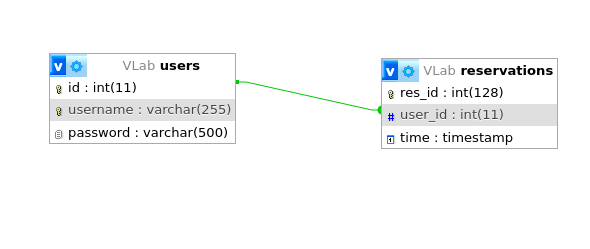
\includegraphics[width=0.8\linewidth]{obrazky-figures/VirtualBoxVM_attUCmGkYe.png}
    \caption{Štruktúra databázy}
\end{figure*}

\subsection{Popis tabuliek}

Tabuľka \verb|VLab users| uchováva informácie o~používateľoch systému \verb|VLab| a~zahŕňa nasledujúce polia:

\begin{itemize}
    \item \verb|id|: Primárny kľúč typu celého čísla (\verb|int(11)|), ktorý jednoznačne identifikuje každého používateľa. Tento atribút je nastavený tak, aby automaticky narastal, čo znamená, že sa automaticky generuje jedinečná hodnota pre každý nový záznam.
    \item \verb|username|: Pole reťazca (\verb|varchar(255)|), ktoré obsahuje používateľské meno používateľa \verb|VLab|. Dĺžka 255 znakov umožňuje široké spektrum používateľských mien. Používateľ sa týmto používateľským menom prihlasuje do systému a~tento atribút je v~databáze nastavený, aby bol unikátnym indexom, čo znamená, že v~danej tabuľke nemôže byť viacej záznamov s~rovnakým používateľským menom.
    \item \verb|password|: Pole reťazca (\verb|varchar(500)|), ukladá heslo pre každého používateľa. Limit 500 znakov je kvôli tomu, že heslá sú uložené v~hašovanej forme, čo je nevyhnutné pre bezpečnosť.
\end{itemize}

Tabuľka \verb|VLab reservations| spravuje rezervácie vytvorené používateľmi v~rámci aplikácie a~zahŕňa nasledujúce polia: 

\begin{itemize}
    \item \verb|res_id|: Primárny kľúč typu celého čísla (\verb|int(11)|), ktorý jednoznačne identifikuje každú rezerváciu. Tento atribút je nastavený tak, aby automaticky narastal, čo znamená, že sa automaticky generuje jedinečná hodnota pre každý nový záznam.
    \item \verb|user_id|: Cudzí kľúč (\verb|int(11)|) spájajúci každú rezerváciu s~používateľom z~tabuľky \verb|VLab users|. Týmto je vytvorený vzťah označujúci, ktorému používateľovi patria jednotlivé rezervácie.
    \item \verb|time|: Pole časovej pečiatky (\verb|timestamp|), ktorá značí začiatok časového úseku, pre ktorý je rezervácia vytvorená.
\end{itemize}

\subsection{Systém správy databáz}

Databáza využíva \verb|MariaDB|, populárny open-sourcový systém na správu relačných databáz. Je to \verb|fork MySQL| a~je známy pre svoj výkon, spoľahlivosť a~jednoduché použitie. \verb|MariaDB| podporuje pokročilé funkcie jazyka \verb|SQL| a~je plne kompatibilná s~\verb|MySQL|, čo znamená, že dokáže spúšťať aj aplikácie napísané pre \verb|MySQL|, a~to bez úprav.

Systém \verb|MariaDB| na správu databázy je dobrou voľbou pre webové aplikácie vďaka svojmu robustnému výkonu. Jeho škálovateľnosť a~pokročilé možnosti klastrovania sú predurčené pre aplikácie, ktoré očakávajú veľké zaťaženie alebo vyžadujú vysokú dostupnosť.

\subsection{Implementácia vzťahov}

Vzťah medzi \verb|VLab users| a~\verb|VLab reservations| je implementovaný prostredníctvom cudzieho kľúča (\verb|user_id|) v~tabuľke  \verb|VLab reservations|, ktorý odkazuje na pole \verb|id| v~tabuľke \verb|VLab users|. Ide o~vzťah typu jedného k~viacerým (\verb|one-to-many|), kde každý používateľ môže mať viacero rezervácií, ale každá rezervácia je spojená iba s~jedným používateľom.

\verb|MariaDB| vynucuje referenčnú integritu pomocou obmedzení cudzích kľúčov. To zaisťuje, že všetky hodnoty \verb|user_id| v~tabuľke \verb|VLab reservations| zodpovedajú existujúcim hodnotám \verb|id| v~tabuľke \verb|VLab users|, čím sa zabráni osamoteným záznamom a~zachová sa konzistencia údajov.

\section{Rozhranie pre správu a~komunikáciu s~PYNQ jednotkami}

Démon je kľúčovou súčasťou systému, zodpovednou za správu komunikácie medzi serverovou aplikáciou a~koncovými zariadeniami PYNQ, vytvára teda medzivrstvu medzi serverovou aplikáciou a~nastavením hosťovského a~serverového systému. Hlavné funkcie démona zahŕňajú:

\begin{itemize}
    \item Získavanie a~poskytovanie informácií o~zariadeniach PYNQ a~vytvorených tuneloch. Démon tieto informácie ukladá v~pamäti a~sú dostupné prostredníctvom REST API endpointov.
    \item Komunikácia s~PYNQ zariadeniami na ich prípravu pre používateľov, čo zahŕňa montovanie používateľských pracovných priečinkov a~konfiguráciu tunelových spojení.
\end{itemize}

Démon komunikuje so serverovou aplikáciou pomocou \verb|REST API endpointov| a~s~PYNQ zariadeniami pomocou \verb|SSH klienta|.

Na implementáciu démona bol z dôvodu týchto požiadaviek vybraný programovací jazyk Go. Démon potrebuje mať napríklad prístup k~sieťovým rozhraniam, čo mu jazyk Go umožňuje. Toto rozhodnutie bolo tiež motivované z~dôvodu jednoduchosti jazyka, robustnej štandardnej knižnice a~rozsiahlej podpory vytvárania REST API serverov a~manipulácie s~IP tabuľkami.

\subsection{Štruktúra démona}

Démon je navrhnutý ako monolitická aplikácia v~jazyku Go, pozostávajúca z~jedného balíka \verb|main|, ktorý obsahuje všetky kľúčové súbory potrebné na jeho fungovanie. Jednotlivé súbory sú špecificky určené na rôzne úlohy a~funkcionalitu démona:

\begin{itemize}
    \item \verb|main.go|: Tento súbor je vstupným bodom programu. Inicializuje a~spustí HTTP server a~zabezpečuje správne načítanie základnej konfigurácie.
    \item \verb|apilib.go|: Definuje štruktúry dát, ktoré démon používa. Tieto štruktúry sú kľúčové pre ukladanie dát o~zariadeniach PYNQ, tunelových spojeniach a~konfiguračných parametroch.
    \item \verb|boot.go|: Obsahuje funkcie, ktoré sa automaticky spustia pri štarte démona. Tieto funkcie zahŕňajú nastavenie IP tabuliek a~načítanie dát o~zariadeniach PYNQ.
    \item \verb|get.go|: Obsahuje implementáciu funkcií, ktoré reagujú na HTTP GET požiadavky od klientov. Tieto funkcie sú zavolané cez definované REST API endpointy a~slúžia na získavanie dát o~zariadeniach PYNQ a~tunelových spojeniach.
    \item \verb|post.go|: Podobne ako \verb|get.go|, ale tento súbor obsahuje funkcie reagujúce na HTTP POST požiadavky. Tieto funkcie vytvárajú a~mažú tunelové spojenia a~aktualizujú stav zariadení PYNQ. 
    \item \verb|sshClient.go|: Zahrňuje implementáciu SSH klienta, ktorý je použitý na komunikáciu so zariadeniami PYNQ.
\end{itemize}

\subsection{Hlavné rozhranie démona}

Súbor \verb|main.go| predstavuje vstupný bod programu, ktorý koordinuje jeho operácie. Tento súbor importuje nevyhnutné balíky a~knižnice jazyka Go, deklaruje globálne premenné, a~zodpovedá za inicializáciu komponentov a~nastavenie HTTP servera. Jeho funkcionalita je rozdelená medzi inicializáciu a~konfiguráciu servera.

Na začiatku súboru sú importované základné balíčky jazyka Go a~knižnice pre vytvorenie HTTP servera, prácu s~IP tabuľkami a~SSH klientom. Súbor následne definuje globálne premenné, ktoré ukladajú informácie o~jednotlivých zariadeniach PYNQ, tunelových spojeniach, konfigurácii a~SSH klientovi.

Pri spustení hlavnej funkcie programu sa najprv inicializuje \verb|iptables| klient a~overí sa jeho funkčnosť. Následne sa načítajú konfiguračné dáta zo súboru, správne nastaví hosťovské prostredie a~inicializuje HTTP server s~definovanými cestami pre REST API endpointy. Tento server je nakoniec spustený na porte 20000 a~počúva prichádzajúce žiadosti, ktoré spracováva podľa priradených definovaných obsluhujúcich funkcií. Na tento server sa nepripojuje klientska časť priamo, ale vždy pristupuje cez serverovú časť webového prostredia, čo zjednodušuje požiadavky na démona.

\subsection{Dátové štruktúry}

Súbor \verb|apilib.go| definuje základné dátové štruktúry, ktoré slúžia na ukladanie dát o~zariadeniach PYNQ, tunelových spojeniach, inštrukcií používateľov a~komunikáciu v~rámci aplikácie. Tieto štruktúry sú serializované do formátu JSON pre sieťový prenos a~sú základom pre aplikačné programové rozhranie (API). Definovaných je šesť dátových štruktúr:

\begin{itemize}
    \item \verb|FPGA|: Ukladá informácie o~jednotlivých zariadeniach PYNQ. Zaznamenáva podstatné informácie ako IP adresu zariadenia, port, ktorý špecifikuje komunikačný kanál a~stav zariadenia. 
    \item \verb|Tunnel|: Reprezentuje informácie o~tunelových spojeniach medzi klientom a~PYNQ zariadeniami. Uchováva údaje ako IP adresy zariadenia a~klienta, ID používateľa a~port používaný pre tunel.
    \item \verb|Instruction|: Definuje formát príkazov posielaných cez API na ovládanie tunelových spojení. Umožňuje špecifikovať akciu (vytvorenie alebo zrušenie), cieľové zariadenie a~používateľa.
    \item \verb|State|: Slúži na zmenu stavu PYNQ zariadenia cez API. Umožňuje dynamicky meniť stav zariadení. Zahrňuje IP adresu zariadenia a~požadovaný stav.
    \item \verb|ErrorInternal|: Táto štruktúra je používaná pre interné chybové hlásenia v~systéme. 
    \item \verb|Commons|: Obsahuje konfiguračné nastavenia, ktoré sú globálne pre celú aplikáciu. Zahrňuje nastavenia sieťových rozhraní a~štartovací port pre maškarádu, ktoré sú potrebné pre správne fungovanie démona a~jeho schopnosť komunikovať s~externými zariadeniami.
\end{itemize}

Dáta v~týchto štruktúrach sú ukladané priamo v~RAM pamäti démona s~tým, že dáta o~PYNQ zariadeniach sú načítané z~konfiguračného JSON súboru. 

\subsection{Konfiguračný súbor}

Máme konfiguračný JSON súbor, ktorý obsahuje dáta o~jednotlivých zariadeniach PYNQ, tento súbor je načítaný pri spustení aplikácie a~dáta z~neho sú serializované do štruktúry \verb|FPGA| a~uložené v~pamäti RAM démona.

\subsection{Práca so sieťovým rozhraním a~tunelmi}

Démon spravuje a~riadi sieťovú komunikáciu medzi klientmi a~zariadeniami PYNQ. Hlavné funkcie zabezpečujú, že komunikácia je efektívne presmerovaná a~bezpečne spravovaná.

\subsubsection*{Počiatočné nastavenie hosťovského prostredia}

Démon obsahuje funkcie na nastavenie a~správu sieťových pravidiel pomocou IP tabuliek, ktoré sú potrebné na riadenie prichádzajúcej a~odchádzajúcej sieťovej komunikácie s~PYNQ zariadeniami. Funkcia \verb|masqueradeCreate()| nastavuje pravidlá pre maškarádu, čo umožňuje, aby odchádzajúca komunikácia zo zariadení PYNQ vyzerala, akoby prichádzala priamo zo servera, na ktorom je démon spustený. Táto funkcia taktiež inicializuje pravidlá na presmerovanie portov, čo umožňuje presnú distribúciu sieťovej komunikácie na špecifické zariadenia pomocou komunikačných kanálov.

Funkcia \verb|tablesFlush()| zase zabezpečuje, že pri spustení aplikácie sa všetky predchádzajúce nastavenia IP tabuliek vymažú. Týmto sa predchádza akumulácii zastaraných alebo konfliktných pravidiel, ktoré by mohli ovplyvniť výkon alebo bezpečnosť aplikácie.

\subsubsection*{Práca s~tunelmi}

Tunely sú vytvárané a~spravované pomocou dvoch kľúčových funkcií: \verb|instructionCreate()| a~\verb|instructionDelete()|, ktoré sú volané podľa typu prijatej inštrukcie cez endpoint. Tieto funkcie riadia vytváranie a~rušenie tunelov, ktoré umožňujú pripojenie medzi klientmi a~PYNQ zariadeniami.

Funkcia \verb|instructionCreate()| spracúva žiadosti o~vytvorenie tunela. To zahŕňa nastavenie príslušných pravidiel v~IP tabuľkách, vytvorenie komunikačného kanálu na porte na serveri pre konkrétneho klienta, a~inicializáciu SSH spojenia pre správu zariadenia PYNQ. Vytvorené tunely sú potom uložené v~globálne dostupnom zozname, čo umožňuje ich ďalšie spracovanie a~poskytovanie dát tunelov pre serverovú aplikáciu.

Na druhej strane, funkcia \verb|instructionDelete()| sa zaoberá rušením tunelov. Tento proces zahŕňa odstránenie pravidiel IP tabuliek, inicializáciu SSH spojenia a~vyčistenie zariadenia PYNQ. Výsledkom je, že zariadenie je pripravené na ďalšie použitie bez dát predošlého používateľa, alebo zanechaných tunelových spojení ostatných používateľov.

Pri vytváraní alebo rušení tunelového spojenia je potrebné, aby sa démon pripojil k~zariadeniu PYNQ a~toto zariadenie pripravil pre používateľa. Na akcie, ktoré je potrebné pri vytváraní alebo rušení tunelového spojenia vykonať, sú vytvorené skripty, ktoré tieto akcie vykonajú a~démon ich len pomocou spojenia spustí. Toto spojenie medzi démonom a~zariadením sa vytvorí cez SSH kanál, ktorý nie je pre používateľov normálne dostupný. Autentifikácia prebieha pomocou RSA kľúča, ktorý je uložený jedine na hosťovskom serveri. Pri eskalácii práv na PYNQ zariadeniach tak nehrozí to, že by niekto dostal prístup ku všetkým zariadeniam.

\section{Systémové požiadavky}

Táto sekcia popisuje nevyhnutné systémové požiadavky na spustenie a~správne fungovanie aplikácie. Aplikácia beží na operačnom systéme \verb|Ubuntu 22.04| so systémom správy databáz \verb|MariaDB|. Webová stránka beží pomocou aplikácie \verb|Apache| a~jazykom PHP, pre ktorý je potrebné rozšírenie \verb|zip|. Démon beží pomocou jazyka \verb|Go|, ktorý má svoje závislosti uložené pomocou balíčkov. Webová aplikácia má závislosti spravované pomocou nástroja \verb|composer|, ktorý ich nainštaluje. Aplikácia potrebuje mať zapnutý a~nastavený \verb|nfs| server.

Pred spustením aplikácie je potrebné, aby server mal vygenerované kľúče pre SSH komunikáciu a~admin nastavil cestu k~týmto kľúčom v~súbore \verb|main.go| v~démonovi a~tak isto nastavil cestu k~priečinku, v~ktorom budú uložené pracovné priečinky používateľov. Túto cestu je potrebné nastaviť jednak v~súbore \verb|main.go| v~démonovi, jednak v~module \verb|FileManager.php| vo funkcii \verb|buildDir()|. Je potrebné túto cestu k~priečinku povoliť pre \verb|nfs| server pre sieť, na ktorej sú pripojené zariadenia PYNQ. 

Pre správne fungovanie aplikácie je potrebné, aby na serveri a~zariadeniach PYNQ bol vytvorený používateľ \verb|student| s~takým istým \verb|UID| na oboch zariadeniach. A~je potrebné, aby bola pod týmto používateľom spustená serverová aplikácia.   

\section{PYNQ nastavenia}

Zariadenie PYNQ je potrebné nastaviť tak, aby správne fungovalo s~aplikáciou. Je potrebné, aby každé zariadenie PYNQ malo pridaný SSH kľúč servera, na ktorom beží aplikácia a~malo povolené, aby server pod týmto kľúčom mohol byť prihlásený bez zadávania hesla ako používateľ \verb|root|, ktorý potom spustí skripty.

Je potrebné, aby skripty (\verb|mount.sh| a~\verb|unmount.sh|), ktoré sa démon pomocou \verb|SSH| spojenia pokúsi, spustiť boli v~domovskom priečinku používateľa \verb|root|.

V~konfiguračnom súbore \verb|jupyter_notebook_config.py|, ktorý sa nachádza v~domovskom priečinku používateľa \verb|root|, je potrebné pridať niekoľko nastavení pre správne fungovanie s~aplikáciou.

\begin{itemize}
    \item Nastavenie nootebookového priečinku na priečinok \verb|/home/student|, na tento priečinok sa budú pripájať pracovné priečinky zo servera. 
    \item Nastavenie terminálu v~Jupyter Notebooku tak, aby pri vytvorení nového terminálu bol prihlásený používateľ \verb|student|.
    \item Nastavenie hesla do Jupyter Notebooku, pomocou ktorého sa prípadní používatelia budú môcť prihlásiť.
    \item Nastavenie čísla portu, na ktorom Jupyter Notebook beží.
    \item Nastavenie cookies \verb|Tornado| web serveru tak, aby stránka Jupyter Notebooku povoľovala \verb|cross-site scripting (XSS)| a~tým umožnila byť vložená do stránok webovej aplikácie.
\end{itemize}




\chapter{Vyhodnotenie vlastností systému na vzorke užívateľov} 
\label{testovanie}

Táto kapitola sa zameriava na vyhodnotenie kľúčových vlastností systému na vzorke reálnych užívateľov. Pochopenie toho, ako koncoví používatelia interagujú so systémom a~aké majú z~neho pocity, je dôležité pre ďalšie smerovanie a~vývoj produktu. Cieľom tohto hodnotenia nie je len overiť funkčnosť a~bezpečnosť systému, ale aj zároveň poskytnúť pohľad na použiteľnosť a~používateľské pohodlie, ktoré systém prináša.

Na začiatku kapitoly je definovaný spôsob, akým bol systém testovaný, ako aj kritériá, podľa ktorých boli vybraní účastníci testovania. Ďalšie sekcie sa venujú rozboru spätnej väzby účastníkov, rozboru výsledkov a~ich implikáciám pre budúce verzie systému. V~závere kapitoly sumarizujem kľúčové zistenia a~formulujem odporúčania pre ďalší vývoj a~zlepšenie systému.

Cieľom tejto kapitoly je poskytnúť komplexný prehľad o~tom, ako je systém vnímaný jeho koncovými užívateľmi a~ako je na tom systém z bezpečnostnej a~funkčnej stránky.

\section{Ciele testovania}

Sekcia si kladie za cieľ detailne definovať a~vymedziť hlavné zámery a~očakávania spojené s~testovaním systému na vybranej vzorke používateľov. Tieto ciele nám pomôžu lepšie pochopiť, ako systém slúži koncovým používateľom, a~sú základom pre interpretáciu získanej spätnej väzby. Hlavné ciele testovania sú:
\begin{itemize}
    \item \verb|Použiteľnosť|: Otestovať, ako intuitívne a~jednoducho môžu používatelia interagovať so systémom pri vykonávaní bežných úloh. Zameriam sa na to, ako rýchlo a~efektívne používatelia dosahujú svoje ciele, a~identifikujem prípadné bariéry, ktoré im v~tom bránia. 
    \item \verb|Spokojnosť používateľov|: Zistiť, do akej miery sú používatelia spokojní s~celkovou funkčnosťou a~klientskym rozhraním aplikácie.
    \item \verb|Bezpečnosť|: Ohodnotiť, ako efektívne aplikácia chráni používateľské dáta a~zabezpečuje prevádzku proti potenciálnym bezpečnostným hrozbám. 
    \item \verb|Adaptabilita|: Posúdiť, ako ľahko je možné systém prispôsobiť zmenám v~požiadavkách na rôzne potreby používateľov.
\end{itemize}

Výsledky získané v~rámci týchto cieľov umožňujú identifikovať silné a~slabé stránky systému, čo je nevyhnutné pre jeho ďalší vývoj, zdokonalenie a~vyhodnotenie bezpečnosti systému.

\section{Postupy použité na testovanie systému}

Vybraná vzorka používateľov zahŕňa troch aktuálnych študentov predmetu IVH a~piatich úspešných absolventov tohto predmetu. Tým je zaručené, že používatelia majú dostatočné technické zručnosti na ohodnotenie implementovaného systému. Používatelia systém testovali pod dohľadom pre bližšie pochopenie pracovného toku používateľa, ktorý používa systém. S~používateľmi bol následne po otestovaní vykonaný rozhovor, v~ktorom som zisťoval odpovede na jednotlivé ciele testovania. 

\section{Výsledky testovania}

Na základe pozorovania používateľov pri práci so systémom a~následnými rozhovormi s~používateľmi bolo zistené, že väčšina cieľov testovania bola pozitívne naplnená. Každý používateľ si pochvaľoval interaktívne používateľské rozhranie a~funkcie systému, ktoré mu umožňujú správu súborov aj mimo rezervovaného časového úseku, alebo jednoduchý a~prehľadný systém na rezerváciu časových úsekov. Používatelia sa snažili použiť \verb|SQL injection| na narušenie systému pri prihlasovaní, alebo pomocou Jupyter Notebooku narušiť zariadenie PYNQ,  pomocou ktorého chceli rozbiť celý systém. 

Vrámci spätnej väzby používatelia požadovali niekoľko zmien na vylepšenie práce s~aplikáciou. Požadovali pridanie počítadla času na navigačnú lištu, ktoré by ukazovalo zostávajúci čas do najbližšej rezervácie, alebo čas do konca aktuálnej rezervácie. Ďalej navrhli pridať potvrdzovací formulár pri mazaní neprázdnych priečinkov v~rozhraní na správu súborov. A~následne aj možnosť si zaregistrovať aktuálne prebiehajúci časový úsek, ak je v~ňom voľné zariadenie PYNQ. Tieto požiadavky som už do aplikácie nestihol implementovať.

\section{Diskusia o výsledkoch}

V~kontexte cieľov testovania bola použiteľnosť a~adaptabilita naplnená. Systém možno na základe spätnej väzby veľmi jednoducho a~intuitívne používať. Systém je možné na základe požiadaviek používateľov zo spätej väzby vďaka rámcu Nette a~JavaScriptu jednoducho rozšíriť o~požadované požiadavky v~ďalších verziách. 

Systém nebolo možné narušiť pomocou \verb|SQL injection| vo formulári na prihlásenie, lebo o~komunikáciu s~databázou sa stará rámec Nette, ktorý správne pracuje so zaslanými dátami vo formulári, takže pri komunikácii s~databázou nedôjde k~\verb|SQL injection|.

Používateľovi sa podarilo narušiť zariadenie PYNQ pomocou Jupyter Notebooku, ktorý beží na zariadení PYNQ pod eskalovanými právami, takže každý Jupyter dokument, ktorý je ním spustený, sa vykonáva s~eskalovanými právami. Toto používateľovi umožnilo narušiť súborový systém zariadenia a~tým vyradiť zariadenie z~prevádzky, ale k~vyradeniu viacerých zariadení pomocou tohto zariadenia sa nedostal, vďaka bezpečnostným opatreniam. Tento problém je možné riešiť logovaním každej akcie používateľa na zariadení a~následným prípadným zamedzením prístupu do systému, čo je možné, keďže systém bude používaný na akademickej pôde, kde používateľmi sú študenti daného predmetu.

\section{Zhrnutie výsledkov}

V~rámci testovania systému boli získané pozitívne ohlasy od používateľov, ktorí si cenili interaktívne užívateľské rozhranie a~pokročilé funkcie systému. Používatelia vyskúšali rôzne bezpečnostné testy, vrátane pokusov o~\verb|SQL injection|, no systém sa ukázal ako odolný vďaka použitiu rámca Nette, ktorý efektívne zamedzil týmto hrozbám. Avšak, bol identifikovaný problém s~eskalovanými právami v~Jupyter Notebooku na zariadeniach PYNQ, ktoré umožnili narušenie súborového systému.

Spätná väzba od užívateľov poukázala na niekoľko oblastí na zlepšenie, vrátane pridania časového počítadla, potvrdzovacieho formulára na mazanie neprázdnych priečinkov a~možnosti rezervácie prebiehajúceho časového úseku, čo zvýši užívateľský komfort pri práci s~aplikáciou. Systém sa javí ako dobre adaptabilný a~ľahko rozšíriteľný na základe užívateľských požiadaviek, čo predstavuje silnú východiskovú pozíciu pre ďalšie vývojové cykly. Celkovo, hoci boli identifikované určité rizikové aspekty, výsledky testovania potvrdili, že systém má solídny základ pre akademické využitie a~ponúka robustné riešenie pre použitie vo výučbe predmetu IVH.

\chapter{Záver}

Cieľom práce bolo vytvoriť aplikáciu virtuálneho laboratória, ktorá umožňuje viacerým používateľom pristupovať k~zdieľaným zariadeniam PYNQ, pomocou tunelových spojení na jednotlivé zariadenia. Pre splnenie tohto cieľa bolo potrebné použiť niekoľko rôznych technológií a~postupov. Tento cieľ bol splnený.

Teoretické vedomosti ohľadom možností zdieľania prostriedkov viacerým používateľom a~vedomosti o~doskách Zynq s~nadstavbou PYNQ som naštudoval a~opísal v~kapitolách \ref{prostriedky} a~\ref{Zynq}. Návrh aplikácie je popísaný v~kapitole \ref{Navrh} a~implementácia aplikácie v~kapitole \ref{Implementacia}. A napokon, vyhodnotenie vlastností implementovaného systému na vzorke používateľov je opísané v~kapitole \ref{testovanie}.

Aplikácia dokáže obsluhovať požiadavky používateľov, vytvárať rezervácie pre časové úseky, pripravovať zariadenia PYNQ pre používateľov, spravovať používateľské súbory uložené na serveri, vytvárať tunelové spojenia na jednotlivé koncové zariadenia PYNQ, spravovať dané zariadenia PYNQ a~rezervácie používateľov pomocou administračného rozhrania.

Hlavným prínosom tejto práce je zjednodušenie prístupu k~zariadeniam PYNQ pomocou webovej aplikácie na výučbu predmetu IVH. 

V~rámci tejto práce som sa stretol s~niekoľkými obmedzeniami, ktoré môžu systém ovplyvniť. Po prvé, príprava jedného zariadenia PYNQ pre ďalšieho používateľa trvá približne 25 sekúnd kvôli nutnosti reštartovania aplikácie Jupyter Notebook, čo môže negatívne ovplyvniť pracovný tok používateľa. Pravda, systém bol testovaný len v~kontrolovanom prostredí, čo môže skresliť výsledky v~porovnaní s~jeho použitím v~reálnej prevádzke.  

Ako rozšírenie práce by bolo možné implementovať jednotlivé požiadavky používateľov získané pomocou spätnej väzby. Aplikáciu by bolo možné rozšíriť pridaním funkcie pre automatické rozpoznávanie a~konfiguráciu nových PYNQ zariadení na sieťovom rozhraní, čo by zjednodušilo prácu pri rozširovaní počtu dostupných zariadení v~prípadoch, keď dopyt po aplikácii náhle vzrastie.

Z~bezpečnostného hľadiska by k~aplikácii bolo možné vytvoriť démona, ktorý by bežal na jednotlivých zariadenia PYNQ a~sledoval aktivitu používateľov na zariadeniach. Ak by došlo k~podozrivej aktivite, napríklad ku vypnutiu tohto démona, alebo k narušeniu súborového systému, nahlásil by túto aktivitu aministrátorovi, a~to už buď pomocou rozhrania na serveri, alebo emailovou komunikáciou.  

  \fi
  
  % Kompilace po částech (viz výše, nutno odkomentovat a zakomentovat input výše)
  % Compilation piecewise (see above, it is necessary to uncomment it and comment out input above)
  %\subfile{chapters/projekt-01-uvod-introduction}
  % ...
  %\subfile{chapters/projekt-05-zaver-conclusion}

  % Pouzita literatura / Bibliography
  % ----------------------------------------------
\ifslovak
  \makeatletter
  \def\@openbib@code{\addcontentsline{toc}{chapter}{Literatúra}}
  \makeatother
  \bibliographystyle{bib-styles/Pysny/skplain}
\else
  \ifczech
    \makeatletter
    \def\@openbib@code{\addcontentsline{toc}{chapter}{Literatura}}
    \makeatother
    \bibliographystyle{bib-styles/Pysny/czplain}
  \else 
    \makeatletter
    \def\@openbib@code{\addcontentsline{toc}{chapter}{Bibliography}}
    \makeatother
    \bibliographystyle{bib-styles/Pysny/enplain}
  %  \bibliographystyle{alpha}
  \fi
\fi
  \begin{flushleft}
  \bibliography{projekt-20-literatura-bibliography}
  \end{flushleft}

  % vynechani stranky v oboustrannem rezimu
  % Skip the page in the two-sided mode
  \iftwoside
    \cleardoublepage
  \fi

  % Prilohy / Appendices
  % ---------------------------------------------
  \appendix
\ifczech
  \renewcommand{\appendixpagename}{Přílohy}
  \renewcommand{\appendixtocname}{Přílohy}
  \renewcommand{\appendixname}{Příloha}
\fi
\ifslovak
  \renewcommand{\appendixpagename}{Prílohy}
  \renewcommand{\appendixtocname}{Prílohy}
  \renewcommand{\appendixname}{Príloha}
\fi
%  \appendixpage

% vynechani stranky v oboustrannem rezimu
% Skip the page in the two-sided mode
%\iftwoside
%  \cleardoublepage
%\fi
  
\ifslovak
%  \section*{Zoznam príloh}
%  \addcontentsline{toc}{section}{Zoznam príloh}
\else
  \ifczech
%    \section*{Seznam příloh}
%    \addcontentsline{toc}{section}{Seznam příloh}
  \else
%    \section*{List of Appendices}
%    \addcontentsline{toc}{section}{List of Appendices}
  \fi
\fi
  \startcontents[chapters]
  \setlength{\parskip}{0pt} 
  % seznam příloh / list of appendices
  % \printcontents[chapters]{l}{0}{\setcounter{tocdepth}{2}}
  
  \ifODSAZ
    \setlength{\parskip}{0.5\bigskipamount}
  \else
    \setlength{\parskip}{0pt}
  \fi
  
  % vynechani stranky v oboustrannem rezimu
  \iftwoside
    \cleardoublepage
  \fi
  
  % Přílohy / Appendices
  \ifenglish
    \input{projekt-30-prilohy-appendices-en}
  \else
    % Tento soubor nahraďte vlastním souborem s přílohami (nadpisy níže jsou pouze pro příklad)

% Pro kompilaci po částech (viz projekt.tex), nutno odkomentovat a upravit
%\documentclass[../projekt.tex]{subfiles}
%\begin{document}

% Umístění obsahu paměťového média do příloh je vhodné konzultovat s vedoucím
\chapter{Obsah priloženého pamäťového média}
Príloha obsahuje dátovú štruktúru priloženého média a popis jednotlivých priečinkov a súborov.

\begin{itemize}
    \item \verb|xvesel92.pdf| - Verzia bakalárskej práce vo formáte PDF.
    \item \verb|xvesel92/| - Priečinok obsahujúci zdrojové kódy pre textovú časť bakalárskej práce.
    \item \verb|daemon/| - Priečinok obsahujúci zdrojové kódy démona.
    \item \verb|Scripts/| - Priečinok obsahujúci skripty, ktoré sa používajú na zariadeniach PYNQ.
    \item \verb|web/| - Priečinok obsahujúci zdrojové kódy webovej aplikácie.
    \item \verb|VLab.sql| - Zdrojový kód generujúci databázu.
    \item \verb|README.md| - Informácie o aplikácii, inštalácie a spustení.
\end{itemize}



%\chapter{Manuál}

%\chapter{Konfigurační soubor}

%\chapter{RelaxNG Schéma konfiguračního souboru}

%\chapter{Plakát}

  \fi
  
  % Kompilace po částech (viz výše, nutno odkomentovat)
  % Compilation piecewise (see above, it is necessary to uncomment it)
  %\subfile{projekt-30-prilohy-appendices}
  
\end{document}
